\documentclass[11pt,a4paper]{article}
\usepackage{fontspec}
\setmainfont{TeX Gyre Pagella}
\setsansfont{TeX Gyre Heros}
\usepackage[margin=21mm,top=24mm,bottom=23mm,headheight=15pt]{geometry}
\usepackage{amsmath,amssymb,graphicx,booktabs,tabularx,longtable,array,enumitem}
\usepackage[table]{xcolor}
\usepackage{tikz}
\usetikzlibrary{arrows.meta,positioning,calc,fit,backgrounds}
\usepackage[most]{tcolorbox}
\usepackage{fancyhdr,titlesec,hyperref,bookmark,microtype,needspace}
\definecolor{ink}{HTML}{172F3B}
\definecolor{teal}{HTML}{176C73}
\definecolor{rust}{HTML}{AA4F2D}
\definecolor{pale}{HTML}{EDF5F4}
\definecolor{warm}{HTML}{FCF2EB}
\definecolor{muted}{HTML}{576872}
\hypersetup{colorlinks=true,linkcolor=teal,urlcolor=teal,pdftitle={Power Systems Module 1 - Complete Study Notes},pdfauthor={Sudheesh},bookmarksdepth=2}
\urlstyle{same}
\setlength{\parindent}{0pt}
\setlength{\emergencystretch}{3em}
\setlength{\parskip}{4pt plus 1pt}
\setlist{itemsep=3pt,topsep=4pt,leftmargin=1.4em}
\renewcommand{\arraystretch}{1.22}
\newcolumntype{Y}{>{\raggedright\arraybackslash}X}
\newcolumntype{L}[1]{>{\raggedright\arraybackslash}p{#1}}
\pagestyle{fancy}\fancyhf{}
\fancyhead[L]{\footnotesize\sffamily\color{muted}POWER SYSTEMS / MODULE 1}
\fancyhead[R]{\footnotesize\sffamily\color{muted}PCEOT503}
\fancyfoot[L]{\footnotesize\sffamily\color{muted}Generation, storage and load analysis}
\fancyfoot[R]{\footnotesize\sffamily\thepage}
\renewcommand{\headrulewidth}{0.3pt}
\titleformat{\section}{\LARGE\sffamily\bfseries\color{ink}}{\thesection}{0.6em}{}
\titleformat{\subsection}{\large\sffamily\bfseries\color{teal}}{\thesubsection}{0.5em}{}
\titleformat{\subsubsection}{\normalsize\sffamily\bfseries\color{ink}}{}{0pt}{}
\titlespacing*{\section}{0pt}{12pt}{9pt}
\titlespacing*{\subsection}{0pt}{11pt}{5pt}
\titlespacing*{\subsubsection}{0pt}{8pt}{3pt}
\tcbset{enhanced,breakable,boxrule=0.4pt,arc=2pt,left=8pt,right=8pt,top=6pt,bottom=6pt,before skip=6pt,after skip=6pt,fonttitle=\sffamily\bfseries}
\newenvironment{Idea}[1]{\begin{tcolorbox}[colback=pale,colframe=teal,coltitle=white,title={#1}]}{\end{tcolorbox}}
\newenvironment{Caution}[1]{\begin{tcolorbox}[colback=warm,colframe=rust,coltitle=white,title={#1}]}{\end{tcolorbox}}
\newenvironment{Worked}[1]{\begin{tcolorbox}[breakable=false,colback=white,colframe=teal,colbacktitle=pale,coltitle=ink,title={#1}]}{\end{tcolorbox}}
\newcommand{\slides}[1]{{\small\color{muted}\textsf{Class-slide anchor: #1.}}\par}
\newcommand{\chapterstart}[2]{\clearpage\section{#1}\label{#2}}
\newcommand{\checkq}[2]{\begin{tcolorbox}[breakable=false,colback=pale,colframe=teal,coltitle=white,title={Check your understanding}]#1\par\textbf{Answer:} #2\end{tcolorbox}}
\tikzset{block/.style={draw=teal,fill=pale,rounded corners=2pt,align=center,text width=2.65cm,minimum height=1.0cm,font=\small\sffamily},hot/.style={block,draw=rust,fill=warm},arr/.style={-{Stealth[length=2.2mm]},thick,draw=ink},control/.style={arr,dashed,draw=rust}}
\newcommand{\diagramcaption}[1]{\par\smallskip{\small\color{muted}#1}\par}
\widowpenalty=10000\clubpenalty=10000
\begin{document}
\pagenumbering{roman}
\begin{titlepage}
\vspace*{12mm}
{\sffamily\small\color{teal}\textbf{CET S5 / 2024 SCHEME / PCEOT503}}\par
\vspace{16mm}
{\sffamily\fontsize{34}{39}\selectfont\bfseries\color{ink}Power Systems\par Module 1}\par
\vspace{7mm}
{\sffamily\LARGE\color{teal}Complete study notes}\par
\vspace{5mm}
{\Large Generation, energy storage\par and load analysis}\par
\vspace{13mm}
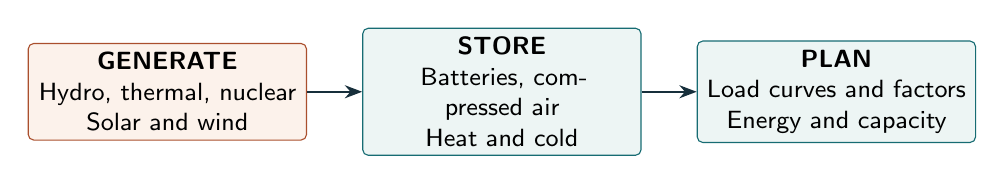
\begin{tikzpicture}
\node[hot,text width=3.3cm] (a) {\textbf{GENERATE}\\Hydro, thermal, nuclear\\Solar and wind};
\node[block,text width=3.3cm,right=7mm of a] (b) {\textbf{STORE}\\Batteries, compressed air\\Heat and cold};
\node[block,text width=3.3cm,right=7mm of b] (c) {\textbf{PLAN}\\Load curves and factors\\Energy and capacity};
\draw[arr] (a)--(b);\draw[arr] (b)--(c);
\end{tikzpicture}
\vspace{12mm}
\begin{Idea}{Built for understanding and exam preparation}
This note covers every Module 1 syllabus item, explaining the physical reasoning and working through all numerical examples. Additional worked examples and practice sets develop independent problem-solving across conventional generation, renewables, energy storage, and power plant economics.
\end{Idea}
\vfill
{\small Comprehensive study notes covering thermal, nuclear, hydro, solar, and wind generation, energy storage, renewable regulations, load curves, and economics according to the 2024-scheme syllabus.}\par\vspace{4mm}
{\small\sffamily Prepared for Sudheesh / 8 October 2026}
\end{titlepage}
\tableofcontents
\clearpage\pagenumbering{arabic}
\chapterstart{Your study map}{roadmap}
\subsection{What Module 1 asks you to learn}
Module 1 has 11 contact hours. Its purpose is to connect \textbf{how electricity is produced}, \textbf{how supply can be shifted in time}, and \textbf{how demand determines the required plant mix}. These three ideas belong together: a technically efficient generator may still be poorly utilised; a large battery may have too little power; a high peak may occur for only a short duration.

\begin{center}\small
\begin{tabularx}{\textwidth}{L{5.8cm}Y}
\toprule\textbf{Every syllabus requirement} & \textbf{Where to study it}\\\midrule
Renewable and non-renewable generation & Foundations, Section~\ref{foundations}\\
Thermal: schematic, environmental / ethical factors, merits and limitations & Section~\ref{thermal}\\
Nuclear: schematic, environmental / ethical factors, merits and limitations & Section~\ref{nuclear}\\
Hydro: schematic, environmental / ethical factors, merits and limitations & Section~\ref{hydro}\\
Solar: schematic, environmental factors, regulations, merits and limitations & Sections~\ref{solar} and \ref{policy}\\
Wind: schematic, environmental factors, regulations, merits and limitations & Sections~\ref{wind} and \ref{policy}\\
BESS, CESS and thermal storage as alternative sources & Section~\ref{storage}\\
Load curve and load-duration curve & Section~\ref{curves}\\
Load, diversity, demand, plant capacity and plant use factors & Section~\ref{factors}\\
Numerical problems & Sections~\ref{classproblems} and \ref{extraexamples}\\\bottomrule
\end{tabularx}\end{center}

\subsection{How to use the note}
\begin{enumerate}
\item \textbf{First reading: understand the energy paths.} For each plant, trace what moves, what heats, what rotates and where electricity leaves. Distinguish material flow from energy transfer.
\item \textbf{Second reading: redraw each schematic without looking.} Label every important component and say why it is needed. A remembered chain of boxes is useful only if its arrows mean something.
\item \textbf{Third reading: solve the class problems yourself.} Hide the solutions; write the time interval, units and denominator before substituting numbers.
\item \textbf{Revision: use Section~\ref{revision}.} Then attempt the questions in Section~\ref{practice}. Answers are included so you can diagnose mistakes.
\end{enumerate}

\begin{Caution}{Core syllabus and added understanding}
Detailed thermodynamic derivations, reactor design calculations, Betz-limit derivation, battery sizing and generation tariffs are not explicitly demanded in this module. Short supporting explanations and clearly marked extension examples are included because they help you understand the class diagrams. Module 2 line parameters and Modules 3--4 protection, faults and stability are outside this note.
\end{Caution}

\subsection{Scope and approach}
This study guide follows the 2024-scheme syllabus for Module 1, integrating physical principles with analytical problem-solving. Diagrams, circuit flows, and plant layouts are presented for clear conceptual understanding, and all class numerical problems are worked through with verification checks.

\chapterstart{Foundations: energy, power and the grid}{foundations}
\slides{Part 1 pp. 1--3, 53, 80, 89--93; Part 2 pp. 1--3, 21--29}
\subsection{Power is a rate; energy is an amount}
\textbf{Power} is the rate of producing or using energy. A 100 MW generator can deliver electrical energy at a rate of 100 megajoules per second. \textbf{Energy} is accumulated power over time:
\[
E=\int_0^T P(t)\,dt,\qquad E=P T\quad\text{for constant power.}
\]
If a 100 MW plant runs at full output for 6 h, it supplies $600\,\mathrm{MWh}$. If it runs at 50 MW for 6 h, it supplies $300\,\mathrm{MWh}$. Its installed rating is still 100 MW.
\begin{Idea}{Units you must keep separate}
$1\,\mathrm{MW}=1000\,\mathrm{kW}$; $1\,\mathrm{MWh}=1000\,\mathrm{kWh}$; one commercial ``unit'' of electricity is $1\,\mathrm{kWh}$. Also, $1\,\mathrm{kWh}=3.6\,\mathrm{MJ}$. A normal 365-day year has 8760 h; a leap year has 8784 h. Ratios of like units are dimensionless.
\end{Idea}

\subsection{Renewable, non-renewable and conventional}
\begin{center}\small
\begin{tabularx}{\textwidth}{L{3cm}YY}
\toprule\textbf{Term} & \textbf{Meaning} & \textbf{Module 1 examples}\\\midrule
Renewable & Replenished by natural processes on relevant human timescales & Hydro, solar, wind; sustainably managed biomass\\
Non-renewable & Uses finite resources depleted by extraction & Coal, oil, natural gas, uranium\\
Conventional & Historically established generation technology & Steam thermal, nuclear and large hydro\\
Variable renewable & Available output depends on changing natural conditions & Solar PV and wind\\\bottomrule
\end{tabularx}\end{center}
\textbf{Conventional is not the opposite of renewable.} Hydro is both conventional and renewable. Nuclear is non-renewable in fuel terms but has low operational carbon emissions. Thermal denotes conversion through heat; it need not mean fossil-fuel combustion. Solar thermal, biomass steam and nuclear plants are all heat-based, though the class uses ``thermal power plant'' mainly for fuel-fired plants.

\subsection{The shared machine, and the important exception}
Most plants in this module drive a generator by rotating a turbine. The source of turbine energy changes:
\begin{itemize}
\item Coal / gas: fuel chemical energy becomes heat.
\item Nuclear: fission energy becomes heat.
\item Hydro: elevated / flowing water supplies hydraulic energy.
\item Wind: moving air supplies mechanical energy.
\end{itemize}
\textbf{Solar PV is the exception}: it converts light directly to DC electricity. It needs an inverter for grid-compatible AC, rather than a boiler or turbine.

A generator converts shaft mechanical power to electrical power through electromagnetic induction. An exciter / field system establishes the magnetic field in a synchronous generator. A transformer changes AC voltage; it does not create energy. Stepping up voltage reduces the current needed for a given transmitted power, helping reduce $I^2R$ losses.

\subsection{Why generation must follow demand}
At the grid boundary, a simplified instantaneous balance is
\[
P_{\rm generation}+P_{\rm imports}+P_{\rm storage,dis}
=P_{\rm load}+P_{\rm losses}+P_{\rm storage,ch}+P_{\rm exports}.
\]
When generation falls short, rotating machines initially give up stored kinetic energy and frequency tends to fall. When generation exceeds demand, frequency tends to rise. Controls, reserves, storage and demand response restore the balance. Exact transient behaviour is studied later in the course.

\begin{Caution}{Interpret ``power cannot be stored'' correctly}
Energy can be stored in batteries, elevated water, compressed air, heat and other forms. The grid conductors do not provide the bulk energy reserve needed for hours of demand. Storage must first be charged, and charging / discharging powers must still fit the instantaneous balance. Stored energy is finite and incurs losses.
\end{Caution}

\subsection{Dispatchability, capacity factor and reliability}
\textbf{Dispatchable} output can be adjusted on command within limits. Reservoir hydro is highly flexible if water is available; coal and nuclear can be controlled but have operating constraints. Wind / PV output depends on the resource, although output can usually be curtailed downward.

\textbf{Capacity factor} measures energy utilisation over a period. It is not a direct reliability score. A peaking plant may deliberately have a low capacity factor and still be essential when demand is highest. Reliability also depends on outages, dependable capacity, reserves, fuel / water availability, transmission and demand patterns.

\textbf{Efficiency} compares useful energy output to energy input. \textbf{Utilisation} compares actual output to an output benchmark. A highly efficient PV module can have a low capacity factor because it is dark at night.

\subsection{How to choose a generation mix}
Choose using the resource, construction / operating cost, demand profile, response speed, emissions, land / water needs, social impact and network connection. Coal / steam and nuclear often supply sustained demand. Reservoir hydro and gas turbines can follow peaks. Solar suits sunny locations and rooftops; wind suits proven high-wind sites. Combining resources, interconnection, demand response and storage improves flexibility. There is no universal ``best plant'' independent of location and the required service.
\checkq{Can a 100 MW solar farm be assumed to supply 100 MW at the evening peak?}{No. Installed capacity is a rating; dependable evening output requires resource assessment and, where appropriate, charged storage or other supply.}

\chapterstart{Thermal generation: steam, gas and combined cycle}{thermal}
\slides{Part 1 pp. 4--24}
\subsection{Working principle of the steam station}
A fuel-fired steam plant converts chemical energy into heat in a furnace. Heat passes through boiler surfaces to water / steam. High-pressure steam expands in a turbine, producing shaft work. The shaft drives an alternator. Exhaust steam is condensed, and a pump returns the liquid water to the boiler.
\[
\text{Fuel chemical energy}\to\text{heat}\to\text{shaft work}\to\text{electrical energy}.
\]
\textbf{The combustion gases and water / steam are different streams.} In normal operation, flue gases heat water through metal surfaces; they do not enter the steam turbine.

\subsection{The three circuits in a steam-plant diagram}
\begin{center}
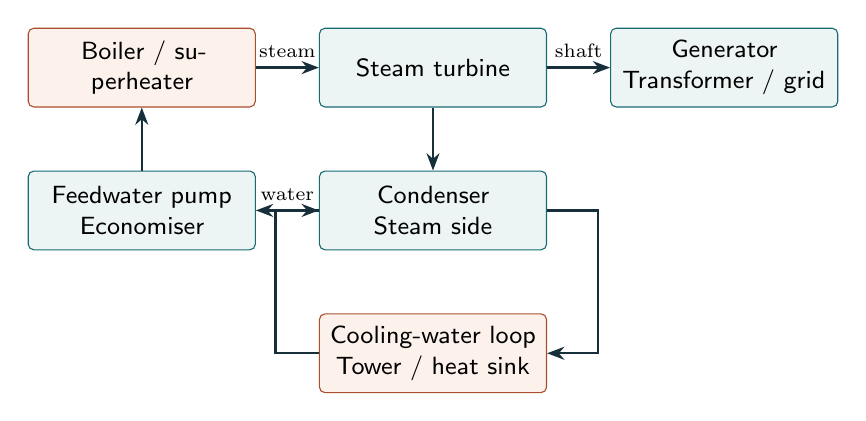
\begin{tikzpicture}[node distance=8mm and 8mm]
\node[hot] (boiler) {Boiler / superheater};
\node[block,right=of boiler] (turb) {Steam turbine};
\node[block,right=of turb] (gen) {Generator\\Transformer / grid};
\node[block,below=of turb] (cond) {Condenser\\Steam side};
\node[block,below=of boiler] (pump) {Feedwater pump\\Economiser};
\node[hot,below=of cond] (cool) {Cooling-water loop\\Tower / heat sink};
\draw[arr] (boiler)--node[above,font=\scriptsize]{steam}(turb);
\draw[arr] (turb)--node[above,font=\scriptsize]{shaft}(gen);
\draw[arr] (turb)--(cond);
\draw[arr] (cond)--node[above,font=\scriptsize]{water}(pump);
\draw[arr] (pump)--(boiler);
\draw[arr] (cond.east)--++(0.65,0)|-(cool.east);
\draw[arr] (cool.west)-|++(-0.55,0.65)|-(cond.west);
\end{tikzpicture}
\end{center}
\diagramcaption{Water / steam circulates in the upper closed loop. Cooling water is a separate stream through the condenser; the diagram shows its supply and return, not mixing with steam.}

\begin{center}
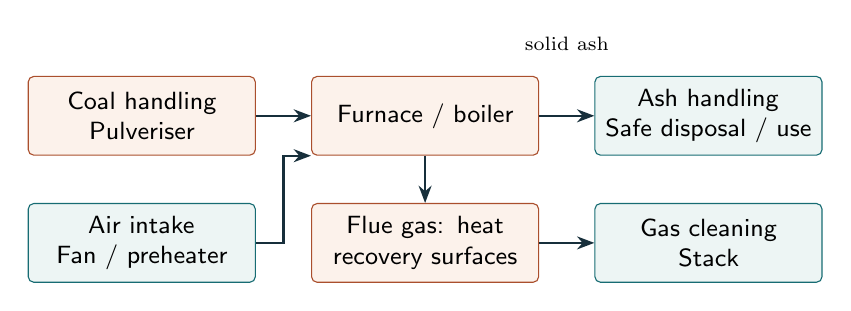
\begin{tikzpicture}[node distance=6mm and 7mm]
\node[hot] (fuel) {Coal handling\\Pulveriser};
\node[hot,right=of fuel] (fire) {Furnace / boiler};
\node[block,right=of fire] (ash) {Ash handling\\Safe disposal / use};
\node[block,below=of fuel] (air) {Air intake\\Fan / preheater};
\node[hot,below=of fire] (flue) {Flue gas: heat\\recovery surfaces};
\node[block,below=of ash] (clean) {Gas cleaning\\Stack};
\draw[arr] (fuel)--(fire);\draw[arr] (air.east)--++(.35,0)|-(fire.south west);
\draw[arr] (fire)--node[above,yshift=7mm,font=\scriptsize]{solid ash}(ash);
\draw[arr] (fire)--(flue);\draw[arr] (flue)--(clean);
\end{tikzpicture}
\end{center}
\diagramcaption{Fuel / ash and air / flue-gas paths. Heat recovery includes superheater, economiser and air-preheater surfaces; their detailed order varies by design.}

\subsubsection{How to narrate the schematic in an exam}
Trace four paths explicitly: (1) coal to furnace and ash disposal; (2) combustion air to furnace, flue-gas heat recovery, cleaning and chimney; (3) pump, boiler, superheater, turbine, condenser and return; (4) cooling-water heat rejection. Then mention turbine-generator coupling and the step-up transformer. This explains a detailed schematic much better than just naming boiler, turbine and generator.

\subsection{Components: what each does and why it matters}
\begin{longtable}{L{3.6cm}L{11.8cm}}
\toprule\textbf{Component} & \textbf{Function and physical reason}\\\midrule\endhead
Coal storage / handling & Receives, stores and conveys fuel. A pulveriser grinds coal to improve contact with air and combustion rate.\\
Boiler / furnace & Fuel burns in the furnace; boiler heat-transfer surfaces produce steam at the required pressure. Water-tube boilers carry water inside tubes; fire-tube boilers carry hot gases inside tubes.\\
Superheater & Raises steam temperature above saturation. This increases available turbine work and reduces moisture in later expansion stages. It does not guarantee completely dry exhaust under every condition.\\
Steam turbine & Successive blade stages extract energy. HP, IP and LP sections indicate high, intermediate and low pressure. Large expansion is spread over stages.\\
Generator & Converts shaft torque and speed to AC electrical output. Generator cooling and excitation support operation.\\
Condenser & Transfers exhaust-steam heat to a cooling medium and condenses steam. Low exhaust pressure increases available expansion / work. Condensation and air-removal equipment maintain the low pressure.\\
Feedwater pump & Raises liquid pressure to boiler pressure. Pumping liquid consumes much less work than compressing the same mass as vapour.\\
Feedwater heater & Uses extracted steam or another heat source to warm feedwater before the boiler; it is distinct from the flue-gas economiser.\\
Economiser & Recovers flue-gas heat into feedwater, reducing fuel needed to reach boiler conditions.\\
Air preheater & Recovers flue-gas heat into incoming combustion air. It heats air, not feedwater.\\
Cooling tower & Rejects heat from circulating cooling water to the atmosphere. It is not the component that directly condenses turbine steam. Once-through cooling or air cooling may replace a tower.\\
Water treatment & Controls scale, corrosion and contamination in the water / steam circuit; makeup water replaces losses.\\
Fans / draught system & Supply air and move combustion gases through the furnace and heat-recovery / cleaning equipment.\\
ESP or filters & Remove particulate fly ash. Sulphur removal requires separate flue-gas desulphurisation; NO$_x$ control uses combustion measures and / or treatment.\\
Chimney / stack & Discharges treated flue gas at height to disperse residual pollutants. Dispersion does not eliminate pollution.\\
Ash handling & Collects bottom ash / fly ash and conveys it for managed disposal or suitable beneficial use.\\\bottomrule
\end{longtable}

\begin{Caution}{Recognise the class photographs}
Part 1 pp. 15--22 show a station, steam-turbine sections, boilers, coal conveyors, a hydraulic runner, a generator, a condenser, cooling towers, a feed pump and governor linkages. A \textbf{steam turbine} is a staged bladed rotor in a casing; a \textbf{water turbine} uses hydraulic energy. The presence of a water-turbine photograph does not make it part of the fossil steam circuit. Identify equipment by its function and fluid, not just its appearance.
\end{Caution}

\subsection{Rankine cycle: understand the closed loop}
The ideal Rankine cycle has four processes:
\begin{enumerate}
\item \textbf{Pump:} liquid water pressure rises; mechanical work is supplied.
\item \textbf{Boiler:} heat is added approximately at constant pressure; water warms, boils and may be superheated.
\item \textbf{Turbine:} steam expands to lower pressure and produces mechanical work.
\item \textbf{Condenser:} heat is rejected approximately at constant pressure, returning steam to liquid.
\end{enumerate}
For understanding only, a steady-flow enthalpy form is
\[
\eta_{\rm cycle}=\frac{(h_3-h_4)-(h_2-h_1)}{h_3-h_2},
\]
with states 1 = condenser exit, 2 = pump exit, 3 = turbine inlet, 4 = turbine exit. The turbine output minus pump input is the net work. The formula is not needed for the syllabus load-factor numericals.

\begin{Idea}{Why condenser heat is not simply avoidable waste}
A heat engine requires a lower-temperature heat sink. The condenser both returns the working fluid to liquid and sets a low turbine exhaust pressure. A cooling tower rejects this heat from the separate cooling-water circuit. Raising steam temperature / pressure and recovering useful heat can improve performance, but no heat engine converts all heat input to electricity.
\end{Idea}

\subsection{Governor and valves: responding to a load change}
In a simple centrifugal governor, rotating weights move outward as speed increases. Linkages alter the steam admission valve. When load increases, electromagnetic torque initially exceeds mechanical torque; speed tends to fall. The governor opens the valve to admit more steam and increase mechanical input. When load decreases, it reduces steam flow.

On an interconnected grid, frequency is a system quantity. A governor adjusts a unit's power contribution and participates in frequency control; it does not independently fix grid frequency exactly. Modern systems commonly use electronic or electrohydraulic governors. The mechanical models in pp. 21--22 illustrate the feedback idea.
\[
N_s=\frac{120f}{p}\quad\Rightarrow\quad N_s=3000\,\mathrm{rpm}
\ \text{for }f=50\,\mathrm{Hz},\ p=2.
\]
Here $p$ is the number of magnetic poles. A 4-pole machine at 50 Hz has a synchronous speed of 1500 rpm.

\subsection{Gas-turbine generation: the open Brayton cycle}
A gas turbine uses air and combustion gas rather than a closed water / steam loop:
\begin{center}
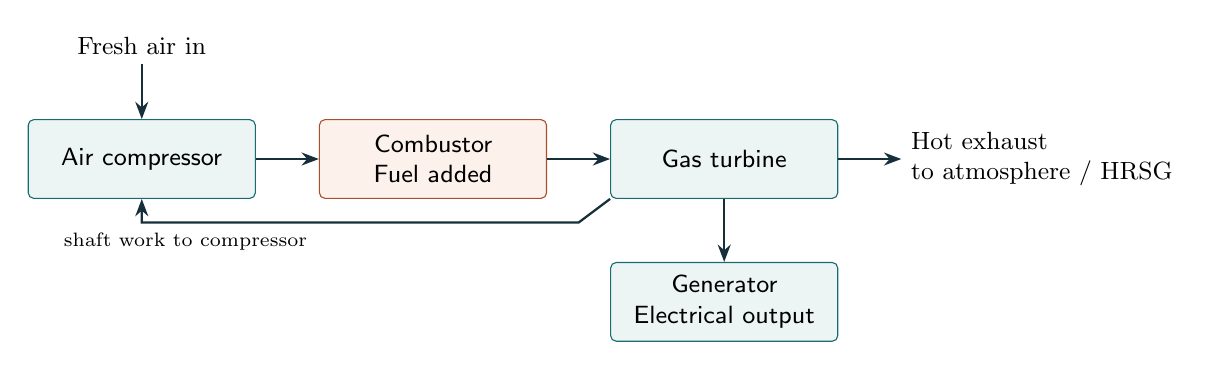
\begin{tikzpicture}[node distance=8mm]
\node[block] (comp) {Air compressor};
\node[hot,right=of comp] (burn) {Combustor\\Fuel added};
\node[block,right=of burn] (gt) {Gas turbine};
\node[block,below=of gt] (g) {Generator\\Electrical output};
\draw[arr] (comp)--(burn);\draw[arr] (burn)--(gt);\draw[arr] (gt)--(g);
\draw[arr] (gt.south west)--++(-0.4,-0.3)-|node[below,font=\scriptsize,pos=.45]{shaft work to compressor}(comp.south);
\node[above=7mm of comp,font=\small] (fresh) {Fresh air in};
\draw[arr] (fresh)--(comp);
\node[right=8mm of gt,font=\small,align=left] (exh) {Hot exhaust\\to atmosphere / HRSG};
\draw[arr] (gt)--(exh);
\end{tikzpicture}
\end{center}
\begin{enumerate}
\item Air is compressed; this consumes a substantial part of turbine work.
\item Fuel burns with compressed air; hot gas is produced.
\item Hot gas expands through the turbine.
\item Turbine work drives the compressor; the remaining shaft work drives the generator.
\end{enumerate}
In an ideal Brayton model, compression and expansion are isentropic and heat addition / rejection occur at constant pressure. A real open-cycle plant takes in fresh air and exhausts gases; the ideal cycle is a thermodynamic model. Fast starting makes simple-cycle gas turbines useful for peak demand and reserves, though fuel cost and efficiency affect dispatch.

\subsection{Combined cycle: use exhaust heat a second time}
\begin{center}
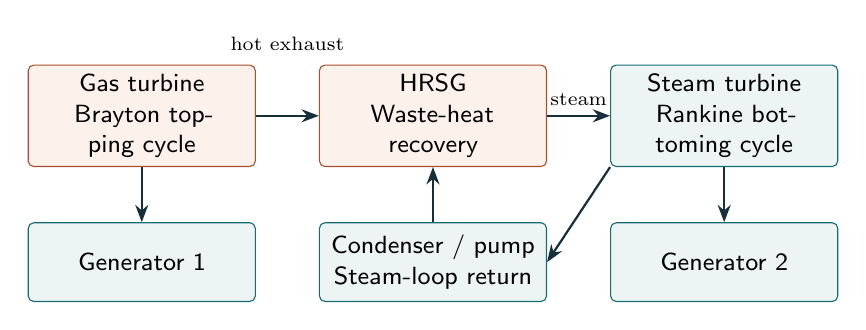
\begin{tikzpicture}[node distance=7mm and 8mm]
\node[hot] (gt) {Gas turbine\\Brayton topping cycle};
\node[hot,right=of gt] (hrsg) {HRSG\\Waste-heat recovery};
\node[block,right=of hrsg] (st) {Steam turbine\\Rankine bottoming cycle};
\node[block,below=of gt] (g1) {Generator 1};
\node[block,below=of st] (g2) {Generator 2};
\node[block,below=of hrsg] (cp) {Condenser / pump\\Steam-loop return};
\draw[arr] (gt)--node[above,yshift=7mm,font=\scriptsize]{hot exhaust}(hrsg);
\draw[arr] (hrsg)--node[above,font=\scriptsize]{steam}(st);
\draw[arr] (gt)--(g1);\draw[arr] (st)--(g2);
\draw[arr] (st.south west)--(cp.east);\draw[arr] (cp)--(hrsg);
\end{tikzpicture}
\end{center}
\diagramcaption{A heat-recovery steam generator (HRSG) transfers exhaust heat to a separate steam loop. Single-shaft arrangements also exist.}
Recovering heat that would otherwise leave in the gas-turbine exhaust raises total output for a given fuel input. Modern high-performance combined-cycle efficiencies can exceed 60\% under specified conditions; that figure is not a guaranteed efficiency for all plants or part-load operation. The turbine exhaust gas does not directly enter the steam turbine.

\subsection{Fuels and the class station examples}
\begin{itemize}
\item \textbf{Coal:} a common steam-station fuel; combustion produces CO$_2$, particulates, sulphur / nitrogen pollutants and ash depending on fuel and controls.
\item \textbf{Natural gas:} common in gas / combined-cycle plants. Lower combustion emissions than coal in comparable electricity production do not make gas emission-free; upstream methane leakage also matters.
\item \textbf{Naphtha:} a light liquid hydrocarbon mixture from refining, used as turbine fuel in suitable equipment.
\item \textbf{Diesel / fuel oil and LSHS:} liquid fuels; Low Sulphur Heavy Stock is a residual petroleum product. The slides describe diesel for starting and LSHS for normal operation at the Kerala examples.
\item \textbf{Biomass:} residues / wood / organic material can be burned or co-fired. Renewable status and climate benefit depend on sustainable sourcing, regrowth, land use and the accounting period.
\end{itemize}
Part 1 p. 14 lists Vindhyachal, Madhya Pradesh (4760 MW); Taichung, Taiwan (5500 MW); Kayamkulam CCPP, Kerala (359 MW); and original capacities of Brahmapuram (106.6 MW) and Kozhikode / Nallalam (128 MW). Retain these as \textbf{class examples}, with dates and boundaries understood.

\begin{Caution}{A factual caution about Kayamkulam}
The slides say it changed from naphtha to pipeline natural gas. NTPC's official RTI Chapter I page, checked on 8 October 2026, describes RGCCPP Kayamkulam as using naphtha as primary fuel [R9]. Therefore this note does not repeat the claimed completed gas switch as a verified fact. The safe learning point is the distinction between liquid-fuel and natural-gas combined-cycle operation.
\end{Caution}

\subsection{Advantages, disadvantages and responsible operation}
\textbf{Advantages:} mature technology; controllable output when fuel and equipment are available; flexible siting compared with large hydro; suitability for large sustained demand. Gas turbines provide faster starting than large steam units. Capital cost and construction duration can be favourable relative to nuclear / large hydro, depending on the project.

\textbf{Disadvantages:} recurring fuel costs, fuel supply risk, fossil depletion, air pollution, greenhouse emissions, ash / waste and cooling-water demand. Large steam units have slow starting, minimum-load / ramp limits and cycling fatigue. Heat rejection reduces overall efficiency.

\begin{center}\small
\begin{tabularx}{\textwidth}{L{4cm}YY}
\toprule\textbf{Impact} & \textbf{Engineering response} & \textbf{Ethical responsibility}\\\midrule
Air pollutants and ash & ESP / filters, FGD, NO$_x$ controls; managed ash use / disposal & Protect neighbours and workers; monitor and report performance\\
CO$_2$ and fuel extraction & Efficient cycles, fuel substitution where justified, reduced demand and transition planning & Consider future generations and local extraction damage\\
Water withdrawal / thermal discharge & Suitable cooling, water reuse, discharge management & Protect competing community water needs and aquatic life\\
Mine / plant closures & Planned retraining and site remediation & Support workers and communities through a just transition\\\bottomrule
\end{tabularx}\end{center}

\subsection{Engineering insights without misleading shortcuts}
The class quotes 540--600$^\circ$C steam, pressures above 25 MPa for advanced units, and ultra-supercritical efficiencies approaching 47\%. These illustrate advanced designs, not every plant. Supercritical water lacks a distinct boiling transition; improved cycle conditions can reduce fuel per kWh.

A cooling-tower plume is predominantly condensed water droplets, not combustion smoke; gaseous water vapour itself is invisible. A ``homes supplied'' estimate needs duration, capacity factor and household demand, not MW rating alone.
\chapterstart{Nuclear generation: controlled fission and heat removal}{nuclear}
\slides{Part 1 pp. 25--39}
\subsection{Fission, chain reaction and criticality}
A neutron absorbed by a fissile nucleus such as uranium-235 can cause it to split into lighter fragments. Energy and further neutrons are released. The released neutrons can cause more fissions: this is a \textbf{chain reaction}. A representative reaction is
\[
{}^{235}_{92}\mathrm{U}+{}^1_0\mathrm{n}
\to{}^{141}_{56}\mathrm{Ba}+{}^{92}_{36}\mathrm{Kr}+3{}^1_0\mathrm{n}+\text{energy}.
\]
This is one possible fragment combination, not the only outcome. Mass / charge balance can be checked: $235+1=141+92+3$ and $92=56+36$. A small mass difference corresponds to released energy through $E=\Delta m c^2$.

The effective multiplication factor $k_{\rm eff}$ describes neutron reproduction from one generation to the next: $k<1$ is subcritical (decreasing), $k=1$ is critical (steady), and $k>1$ is supercritical (increasing). In normal steady operation, ``critical'' means a sustained controlled reaction; it does not mean an accident.

\begin{Idea}{The same downstream heat engine, a different heat source}
\textbf{Nuclear energy $\to$ heat $\to$ mechanical energy $\to$ electrical energy.} A reactor replaces the fuel-fired furnace as the heat source. The steam turbine, generator and condenser perform broadly the same downstream functions as in a steam thermal station.
\end{Idea}

\subsection{Read the nuclear schematic as separate loops}
The class diagrams show a reactor transferring heat through a heat exchanger to a steam loop. A \textbf{pressurised water reactor (PWR)} is a useful concrete model:
\begin{center}
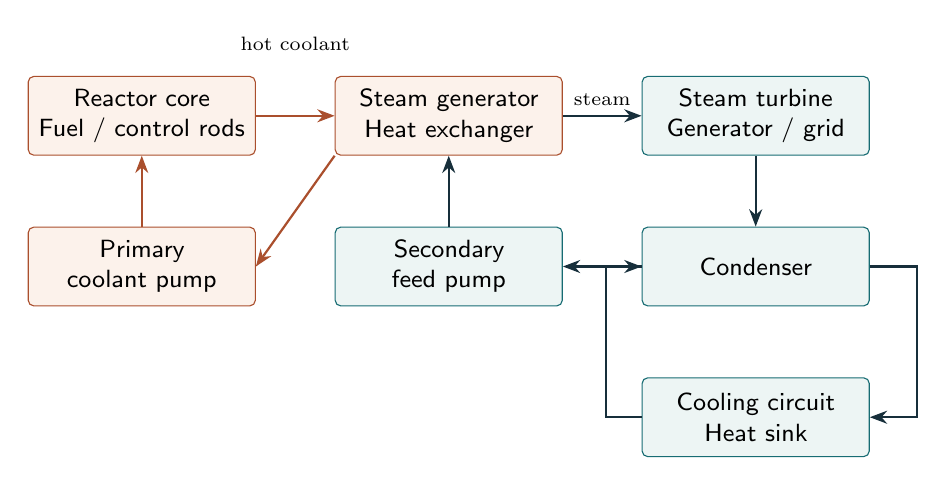
\begin{tikzpicture}[node distance=9mm and 10mm]
\node[hot] (core) {Reactor core\\Fuel / control rods};
\node[hot,right=of core] (sg) {Steam generator\\Heat exchanger};
\node[block,right=of sg] (turb) {Steam turbine\\Generator / grid};
\node[hot,below=of core] (pp) {Primary coolant pump};
\node[block,below=of sg] (fp) {Secondary feed pump};
\node[block,below=of turb] (cond) {Condenser};
\node[block,below=of cond] (cool) {Cooling circuit\\Heat sink};
\draw[arr,draw=rust] (core)--node[above,yshift=7mm,font=\scriptsize]{hot coolant}(sg);
\draw[arr,draw=rust] (sg.south west)--(pp.east);\draw[arr,draw=rust] (pp)--(core);
\draw[arr] (sg)--node[above,font=\scriptsize]{steam}(turb);
\draw[arr] (turb)--(cond);\draw[arr] (cond)--(fp);\draw[arr] (fp)--(sg);
\draw[arr] (cond.east)--++(.6,0)|-(cool.east);
\draw[arr] (cool.west)--++(-.45,0)|-(cond.west);
\end{tikzpicture}
\end{center}
\diagramcaption{The primary and secondary fluids exchange heat but normally do not mix. The condenser's cooling-water circuit is a third stream.}
\begin{enumerate}
\item \textbf{Primary loop:} pressurised coolant transports core heat to the steam generator and returns via the coolant pump. Pressure prevents normal bulk boiling in a PWR.
\item \textbf{Secondary loop:} feedwater receives heat and becomes steam. Steam expands in the turbine, condenses and returns via the feed pump. It does not normally pass through the reactor core.
\item \textbf{Cooling loop:} removes condenser heat to a water body, cooling tower or other heat sink.
\end{enumerate}
A boiling-water reactor (BWR) produces steam in the reactor vessel and has a different circuit. Do not present a two-loop PWR schematic as the layout of every reactor. Water may serve as coolant and moderator; heavy water or graphite is used in other designs.

\subsection{Reactor components you should explain}
\begin{center}\small
\begin{tabularx}{\textwidth}{L{3.4cm}Y}
\toprule\textbf{Part} & \textbf{Role}\\\midrule
Fuel and cladding & Fuel undergoes fission; cladding contains fuel and many fission products while transferring heat.\\
Moderator & Slows neutrons to increase the likelihood of fission in thermal-reactor fuels. It is not a control rod.\\
Control rods & Absorb neutrons to control reactivity; insertion supports shutdown. Boron / cadmium / hafnium compounds are examples.\\
Coolant & Carries heat from the fuel; its function is heat transport.\\
Pressure vessel / channels & Contain the core / coolant at operating conditions, depending on reactor type.\\
Steam generator & Transfers primary-loop heat to the steam-producing loop in indirect-cycle designs.\\
Biological shielding & Reduces radiation exposure around the reactor; concrete and other shielding materials are used.\\
Containment & A barrier designed to limit radioactive release under specified conditions. Shielding and containment have related but different purposes.\\
Safety and cooling systems & Detect abnormal conditions, shut down the chain reaction and remove decay heat, including after loss of normal power.\\\bottomrule
\end{tabularx}\end{center}

\subsection{Why shutdown does not end the need for cooling}
Control rods suppress the chain reaction, but radioactive fission products continue to decay and release heat. This \textbf{decay heat} decreases with time, yet can initially be large enough to damage fuel without cooling. A safe plant therefore needs reliable heat removal and backup power / alternative cooling after shutdown. This is a central design principle in IAEA safety requirements [R8].
\checkq{Are control rods and moderator interchangeable?}{No. Control rods absorb neutrons; a moderator slows them. Both affect the reaction but through different mechanisms.}

\subsection{Advantages and disadvantages}
\textbf{Advantages:} very high fuel energy density; large sustained generation; low greenhouse-gas emissions during operation; small fuel volumes compared with coal; long operating life with appropriate maintenance and licensing. High capacity factors are achievable, but not guaranteed.

\textbf{Disadvantages:} high capital cost; lengthy construction / licensing; specialised operation and safety requirements; spent-fuel and radioactive-waste responsibilities; decommissioning cost; low-probability but serious accident consequences; cooling-water and site constraints.

\subsection{Environmental and ethical factors}
Operational CO$_2$ is low because no carbon fuel is burned for the principal heat source. Lifecycle impacts include uranium mining, processing / enrichment, construction, fuel manufacture, waste and decommissioning. Cooling-water withdrawal and warm discharges can affect aquatic ecosystems.

Waste management requires suitable containment, monitoring and, for relevant waste classes, long-term isolation. The \textbf{intergenerational question} is who bears responsibility and cost after the electricity has been consumed. Ethical practice also requires transparent risk communication, competent independent regulation, emergency preparedness and fair participation of communities in siting decisions. Civilian fuel / materials need safeguards against misuse; this is distinct from ordinary reactor operation.

\subsection{The two class safety case studies}
\begin{Worked}{Chernobyl, Ukraine / then USSR - 26 April 1986}
The class emphasises a safety test, a rapid power excursion, explosions and radioactive release. The lesson is not adequately expressed as ``operator error'' alone: reactor characteristics, procedures, training and safety culture interacted. Contamination and evacuation caused lasting social and environmental disruption.\par
\textbf{Study takeaway:} safe design, independent review, clear operating limits, trained operators and honest reporting are essential. A failure in one reactor design should not be assumed to describe the design of all reactors.
\end{Worked}
\begin{Worked}{Fukushima Daiichi, Japan - 11 March 2011}
An earthquake and tsunami damaged the site's ability to maintain power and cooling. Loss of heat removal after shutdown led to severe fuel damage and hydrogen explosions. The explosions were chemical hydrogen explosions, not a nuclear detonation.\par
\textbf{Study takeaway:} consider extreme external events and common-cause failures; protect diverse backup power and maintain cooling after shutdown. Accident consequences include evacuation, displacement, cleanup and long-term recovery, not only direct radiation effects.
\end{Worked}
The slides quote evacuation counts and make a statement about direct radiation deaths. Those are historical contextual claims with definitions and reporting periods; an exam answer on engineering lessons does not require an unsupported absolute claim about all health consequences.

\subsection{Examples and the ``tiny fuel'' comparisons}
The slides list Kudankulam, Tamil Nadu (2000 MW) and Kashiwazaki-Kariwa, Japan (7965 MW installed). Treat those capacities and rankings as slide-era context; installed capacity and operating availability differ. Reactor, containment and station photographs in pp. 34--35 help you identify the physical barriers and buildings.

Fuel-pellet, lifetime-can and submarine examples in p. 32 illustrate \textbf{high fuel energy density}. Exact coal-equivalent energy or lifetime fuel volume depends on fuel burnup, efficiency and consumption assumptions. Submarine endurance additionally depends on crew supplies and operational constraints. Learn the principle instead of treating the analogies as universal conversion constants.

\chapterstart{Hydroelectric generation: head, flow and control}{hydro}
\slides{Part 1 pp. 40--52}
\subsection{Working principle and hydraulic power}
Water at elevation has gravitational potential energy. A dam / diversion and waterway establish a useful \textbf{head}, the elevation / energy difference across the turbine. Water transfers hydraulic energy to the turbine runner, and its shaft drives a generator. Water returns downstream through the tailrace.
\[
\text{Water head / flow}\to\text{hydraulic flow}\to
\text{mechanical shaft power}\to\text{electrical power}.
\]
The potential-to-kinetic sequence in the slides is especially intuitive for an impulse jet. Reaction turbines also extract energy from pressure changes, so ``all energy first becomes a free jet'' is not the general hydro principle.

For additional understanding,
\[
P_{\rm electrical}=\rho g Q H_{\rm net}\eta_t\eta_g.
\]
$\rho$ is water density (about $1000\,\mathrm{kg / m^3}$), $g=9.81\,\mathrm{m / s^2}$, $Q$ is flow ($\mathrm{m^3/s}$), $H_{\rm net}$ is usable head (m), and $\eta_t\eta_g$ is turbine-generator efficiency. \textbf{Gross head} is the elevation difference; \textbf{net head} subtracts relevant hydraulic losses. Higher head or flow means more available hydraulic power.

\subsection{A schematic with the surge tank in the right place}
\begin{center}
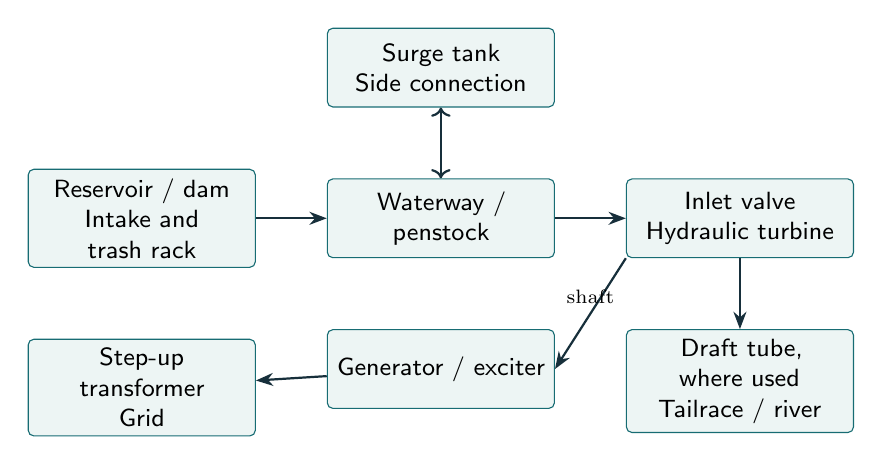
\begin{tikzpicture}[node distance=9mm and 9mm]
\node[block] (res) {Reservoir / dam\\Intake and trash rack};
\node[block,right=of res] (pen) {Waterway / penstock};
\node[block,right=of pen] (turb) {Inlet valve\\Hydraulic turbine};
\node[block,above=of pen] (surge) {Surge tank\\Side connection};
\node[block,below=of turb] (tail) {Draft tube, where used\\Tailrace / river};
\node[block,below=of pen] (gen) {Generator / exciter};
\node[block,below=of res] (grid) {Step-up transformer\\Grid};
\draw[arr] (res)--(pen);\draw[arr] (pen)--(turb);\draw[arr,<->] (pen)--(surge);
\draw[arr] (turb)--(tail);\draw[arr] (turb.south west)--node[above,font=\scriptsize]{shaft}(gen.east);\draw[arr] (gen)--(grid);
\end{tikzpicture}
\end{center}
\diagramcaption{The surge tank is connected to the waterway to exchange water during transients; it is not normally a separate serial energy-conversion stage. Exact waterway arrangement depends on the site.}

\subsection{Components in the class layouts}
\begin{itemize}
\item \textbf{Dam and reservoir:} retain water, create head and permit storage of inflow. The dam itself does not generate electricity.
\item \textbf{Intake, sluice gates and trash racks:} admit / isolate water and screen debris. Screens do not remove every particle of silt.
\item \textbf{Forebay:} an intake basin providing a local supply to the penstock in appropriate layouts.
\item \textbf{Penstock and supports:} pressure conduit to the turbine, designed for hydraulic pressure and transients.
\item \textbf{Surge tank:} reduces rapid pressure changes and supplies / absorbs water while flow adjusts. Sudden valve closure can cause \textbf{water hammer}, a pressure wave in the waterway.
\item \textbf{Turbine:} converts hydraulic energy into shaft power. Inlet valves and guide vanes / nozzles regulate flow.
\item \textbf{Draft tube:} a diverging discharge passage used with reaction turbines to recover part of exit kinetic energy and permit a suitable turbine setting. It is not a standard Pelton-wheel discharge component.
\item \textbf{Tailrace:} conveys discharged water downstream.
\item \textbf{Generator, exciter, transformer and control room:} create electrical output, establish / control excitation, connect at the required voltage and supervise operation.
\end{itemize}

\subsection{Turbine choice and hydro plant types}
\begin{center}\small
\begin{tabularx}{\textwidth}{L{3cm}YY}
\toprule\textbf{Turbine} & \textbf{Physical action} & \textbf{Usual suitability}\\\midrule
Pelton (impulse) & Jet momentum drives buckets; runner is not fully immersed in a pressure casing & High head, relatively low flow\\
Francis (reaction) & Pressure and velocity change through the runner & Broad medium-head applications\\
Kaplan (reaction) & Axial-flow runner, often adjustable blades & Low head, high flow\\\bottomrule
\end{tabularx}\end{center}
These are qualitative guides. Exact head boundaries depend on turbine design and economics, rather than universal cutoffs.

\textbf{Reservoir hydro} stores natural inflow and can schedule release within water constraints. \textbf{Run-of-river} uses current inflow with limited storage and can be more variable. \textbf{Pumped storage} uses electricity to pump water uphill, later releasing it through turbine-generators. Pumped storage is a net energy consumer over a full charge / discharge cycle; it shifts energy in time rather than creating a new primary energy resource.

\subsection{Governor and excitation in the hydro schematic}
The governor changes water admission / guide-vane or nozzle settings to control turbine power and participate in frequency control. Excitation changes the generator field and supports voltage / reactive-power control. These are \textbf{different control tasks}. The feedback in Part 1 p. 42 should be read as a control signal, not another water or electrical power path.

\begin{Worked}{Understanding example: power from a water flow}
For $Q=40\,\mathrm{m^3/s}$, net head $H=100\,\mathrm{m}$ and overall turbine-generator efficiency 0.90,
\[
P=1000(9.81)(40)(100)(0.90)=35.316\times10^6\,\mathrm{W}
=35.32\,\mathrm{MW}.
\]
Doubling net head with the same flow and efficiency doubles this output. This is an extension example; the syllabus numericals focus on loads and factors.
\end{Worked}

\subsection{Advantages, disadvantages and environmental / ethical factors}
\textbf{Advantages:} renewable water-cycle resource; no fuel combustion for normal generation; low fuel cost; long service life; rapid response and useful frequency / peak support; potential irrigation / flood-control benefits. Some suitably designed units can support black start, meaning system restoration without an already energised external grid.

\textbf{Disadvantages:} high civil-work cost and long construction; dependence on site / head / water; drought and seasonal variability; sedimentation and erosion; long network connection at remote sites; dam safety responsibility and reservoir social impacts.

\textbf{Environmental factors:} inundated habitats / farmland, altered river flow and sediment movement, blocked fish migration, water-quality changes and possible reservoir methane from decomposing organic material. Hydro has no fossil combustion in operation; its lifecycle greenhouse emissions are not necessarily zero.

\textbf{Ethical factors:} consent and participation of displaced communities; fair compensation and livelihood rehabilitation; protection of cultural sites; downstream water needs and equitable sharing across regions / countries. Mitigation includes suitable environmental flows, sediment management, fish passage where effective, careful siting and responsible resettlement. Multipurpose use creates competing priorities, so full reservoir power availability cannot always be assumed.

\subsection{The class examples and photographs}
The slides list Tehri, Uttarakhand (1000 MW and dam height 260.5 m); Three Gorges, China (22500 MW); and Idukki, Kerala (780 MW). Idukki's arch dam lies between Kuravan and Kurathi hills; the water supports generation at the Moolamattom powerhouse. The dam photograph and generator photograph are different parts of the project.

The slide analogy about Three Gorges and a tiny change in Earth's rotation illustrates redistribution of mass; it is not a power-generation equation. Water-jet speeds above 100 km / h are illustrative of some heads, not a universal requirement. Quick starting and fish ladders / elevators are useful concepts, but response time and ecological effectiveness are site-dependent.
\checkq{Can a run-of-river station guarantee full output during a dry season just because it is renewable?}{No. Renewable describes replenishment of the resource; dependable output still depends on available water and head.}

\chapterstart{Solar generation: PV and solar thermal}{solar}
\slides{Part 1 pp. 53--67}
\subsection{PV begins in the semiconductor}
A solar cell absorbs suitable photons and creates electron-hole pairs. A p-n junction's built-in electric field separates carriers, and metal contacts collect current through an external circuit. Light absorption and carrier collection occur over the device, not exclusively within the depletion region. The essential idea is \textbf{direct conversion from light to electricity}.

\begin{center}
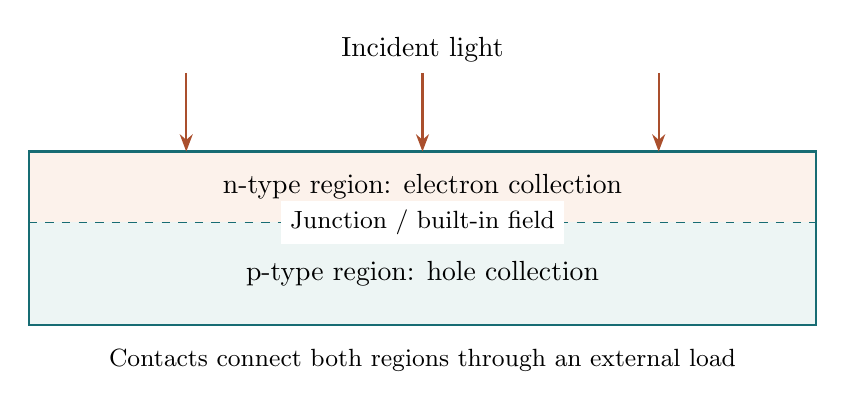
\begin{tikzpicture}
\fill[pale] (0,0) rectangle (10,1.3);
\fill[warm] (0,1.3) rectangle (10,2.2);
\draw[teal,thick] (0,0) rectangle (10,2.2);
\draw[dashed,teal] (0,1.3)--(10,1.3);
\node at (5,1.75) {n-type region: electron collection};
\node at (5,.65) {p-type region: hole collection};
\node[font=\small,fill=white] at (5,1.3) {Junction / built-in field};
\draw[arr,draw=rust] (2,3.2)--(2,2.2);
\draw[arr,draw=rust] (5,3.2)--(5,2.2);
\draw[arr,draw=rust] (8,3.2)--(8,2.2);
\node at (5,3.5) {Incident light};
\node[font=\small] at (5,-.45) {Contacts connect both regions through an external load};
\end{tikzpicture}
\end{center}
\diagramcaption{Conceptual cell cross-section, supporting Part 1 pp. 54--55. Practical layers include front contacts, an anti-reflection layer, semiconductor regions and a back contact.}
An isolated cell gives a small voltage. Cells in \textbf{series} increase voltage; parallel strings increase available current. Cells form modules; modules form arrays. The class panels and floating-array photographs show assemblies, not individual cells. Technical cross-check: DOE PV resources [R4].

\subsection{Grid-connected PV schematic}
\begin{center}
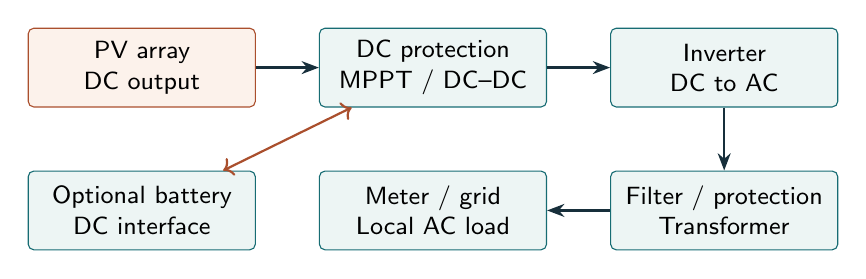
\begin{tikzpicture}[node distance=8mm and 8mm]
\node[hot] (pv) {PV array\\DC output};
\node[block,right=of pv] (dc) {DC protection\\MPPT / DC--DC};
\node[block,right=of dc] (inv) {Inverter\\DC to AC};
\node[block,below=of inv] (filter) {Filter / protection\\Transformer};
\node[block,below=of dc] (grid) {Meter / grid\\Local AC load};
\node[block,below=of pv] (bat) {Optional battery\\DC interface};
\draw[arr] (pv)--(dc);\draw[arr] (dc)--(inv);\draw[arr] (inv)--(filter);\draw[arr] (filter)--(grid);
\draw[arr,<->,draw=rust] (bat)--(dc);
\end{tikzpicture}
\end{center}
\diagramcaption{The battery branch needs a suitable charge / discharge interface. MPPT may be integrated in the inverter; a separate boost converter is not mandatory in every system.}
\begin{itemize}
\item \textbf{PV modules:} generate DC; output changes with irradiance, cell temperature, shading and losses.
\item \textbf{MPPT:} maximum power point tracking adjusts the operating point to extract available panel power as conditions change. It does not create energy or guarantee rated output.
\item \textbf{Inverter:} converts DC into grid-compatible AC and controls injected current. Grid-side filtering reduces switching harmonics; voltage / frequency sensing supports synchronisation and control.
\item \textbf{Transformer:} matches the plant's AC voltage to the collection / transmission network when required.
\item \textbf{Protection and meter:} support safe connection and measurement. Ordinary grid-following rooftop inverters disconnect on loss of the utility grid to avoid unsafe islanding unless specifically designed and permitted for backup operation.
\item \textbf{Mounting structure:} provides orientation and mechanical support; fixed tilt and trackers have different cost / energy tradeoffs.
\end{itemize}
The reactive-power control marked in Part 1 p. 58 means the converter can support voltage within its design / current limits. An inverter's power-electronic interface is not equivalent to automatically having synchronous-machine inertia.

\subsection{Three PV arrangements}
\textbf{Grid connected:} grid supplies deficits and accepts permitted exports; storage is optional. \textbf{Stand-alone:} must balance local supply and demand, often using a charge controller, battery and inverter. \textbf{Hybrid:} combines PV with storage / other generation and suitable controls. A battery drawn in the class diagram is not proof that every PV plant requires one.

\textbf{Floating PV} places arrays on suitable water surfaces. It may reduce land conflict and evaporation, but requires anchoring, corrosion / weather design and water-ecology assessment. Cooler conditions may improve output, depending on the installation. \textbf{Rooftop PV} uses existing surfaces; \textbf{agrivoltaics} combine carefully designed PV with agricultural activity.

\subsection{Solar thermal / concentrating solar power}
Solar thermal electricity uses mirrors to concentrate radiation onto a receiver. A heat-transfer medium carries the heat to storage and / or a steam generator. Steam drives a turbine-generator, and a condenser / pump completes the Rankine loop.
\begin{center}
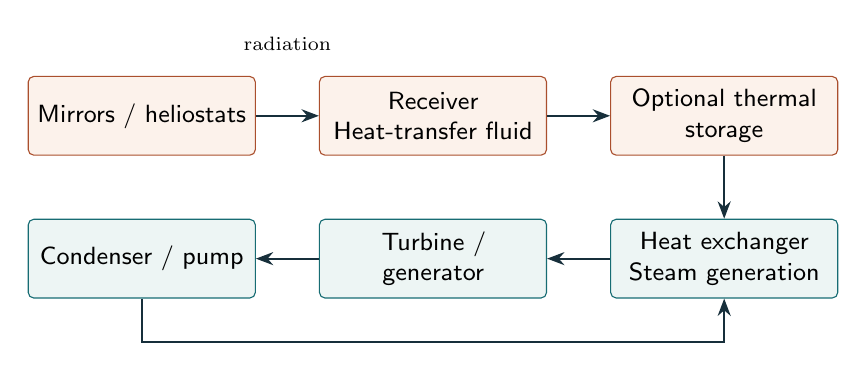
\begin{tikzpicture}[node distance=8mm and 8mm]
\node[hot] (mir) {Mirrors / heliostats};
\node[hot,right=of mir] (rec) {Receiver\\Heat-transfer fluid};
\node[hot,right=of rec] (store) {Optional thermal\\storage};
\node[block,below=of store] (steam) {Heat exchanger\\Steam generation};
\node[block,below=of rec] (turb) {Turbine / generator};
\node[block,below=of mir] (cp) {Condenser / pump};
\draw[arr] (mir)--node[above,yshift=7mm,font=\scriptsize]{radiation}(rec);
\draw[arr] (rec)--(store);\draw[arr] (store)--(steam);\draw[arr] (steam)--(turb);\draw[arr] (turb)--(cp);\draw[arr] (cp.south)--++(0,-.55)-|(steam.south);
\end{tikzpicture}
\end{center}
\diagramcaption{Heat can pass directly from the receiver to the steam generator as well. Flow-return paths on the heat-transfer-fluid side are omitted for clarity.}
\textbf{Parabolic troughs} focus onto receiver tubes; a \textbf{solar tower} uses heliostats to focus onto an elevated receiver. The tower photograph in Part 1 p. 65 illustrates this geometry. Sufficiently charged thermal storage enables generation after sunset, for a finite design duration. Output also needs an operating power block and heat sink. DOE CSP basics cross-check this conversion route [R5].

\begin{center}\small
\begin{tabularx}{\textwidth}{L{3cm}YY}
\toprule\textbf{Feature} & \textbf{PV} & \textbf{CSP / solar thermal electricity}\\\midrule
Conversion & Light directly to DC; inverter for AC & Light to heat, then heat engine / generator\\
Moving machinery & No turbine in PV conversion; trackers may move & Mirrors may track; turbine / pumps operate\\
Storage & Often electrical battery storage & Often heat storage, e.g. molten salt\\
Resource & Can use direct and diffuse light & Concentration relies principally on direct sunlight\\
Water & Mainly cleaning, subject to design & Cleaning and heat rejection; dry cooling can reduce water demand\\
After sunset & No PV generation; stored energy / other source needed & Charged thermal storage can continue generation\\\bottomrule
\end{tabularx}\end{center}

\subsection{Advantages, limitations and environmental factors}
\textbf{PV advantages:} abundant renewable source; no normal fuel cost; no combustion at point of generation; modular rooftop-to-utility deployment; relatively low mechanical maintenance. \textbf{Limitations:} daylight / weather variability, land / network requirements at scale, temperature / shading / soiling losses, and storage / backup needs for required availability.

High sunlight and high temperature are different: higher irradiance generally increases available output, while higher cell temperature commonly reduces silicon-module voltage / efficiency. A hot desert can be an excellent solar location despite temperature penalties. PV has no moving parts in the cells, but inverters and mounting / tracking systems need maintenance.

\textbf{Environmental issues:} material extraction, manufacturing energy / chemicals, land habitat effects, water for cleaning, end-of-life recycling and waste. Floating PV can affect water use / ecology; CSP adds hot-fluid management, heat rejection and possible wildlife effects near concentrated flux. Mitigation means suitable sites, responsible sourcing, efficient water use and recycling plans. Operational emissions are low, not proof of zero lifecycle impact.

\subsection{Notable project examples}
Part 1 shows a field array, the NTPC Harippad / Kayamkulam floating installation and a solar tower. Named examples include Bhadla Solar Park, Rajasthan (2245 MW in the slides); Golmud, Qinghai, China (over 2800 MW in the slides); and Noor Ouarzazate, Morocco, as a major solar-thermal example. These names illustrate different plant types and locations; capacities / rankings change and are not required formula inputs.
\checkq{Why can CSP with heat storage generate after sunset while ordinary PV cannot?}{CSP can feed previously stored heat to a turbine cycle. PV stops converting sunlight when light is unavailable; a PV system can still supply loads from separately charged storage.}

\chapterstart{Wind generation: rotor, converter and controls}{wind}
\slides{Part 1 pp. 68--77}
\subsection{From moving air to shaft power}
Wind is moving air with kinetic energy. Pressure differences around aerofoil blades produce lift and rotor torque. The rotor shaft drives a generator, directly or through gearing. Generated electricity is conditioned and transformed for the grid.
\[
\text{Wind kinetic energy}\to\text{rotor mechanical energy}\to\text{electrical energy}.
\]
Supporting physical relationships are
\[
P_{\rm wind}=\tfrac12\rho A v^3,\quad
P_{\rm rotor}=C_pP_{\rm wind},\quad A=\pi R^2.
\]
Here $\rho$ is air density, $v$ is wind speed, $A$ is swept area and $C_p$ is aerodynamic power coefficient. An ideal isolated rotor cannot extract all wind power: air must continue downstream. The Betz limit is $C_p\le16/27\approx0.593$. Electrical output is further reduced by drive / generator / converter losses and limited by rated power. This relationship is an aid to understanding, not a demand for a detailed derivation in Module 1.

\subsection{Mechanical schematic and nacelle parts}
\begin{center}
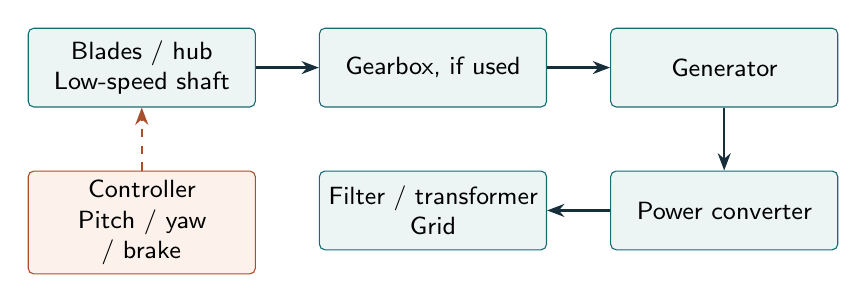
\begin{tikzpicture}[node distance=8mm and 8mm]
\node[block] (rot) {Blades / hub\\Low-speed shaft};
\node[block,right=of rot] (gear) {Gearbox, if used};
\node[block,right=of gear] (g) {Generator};
\node[block,below=of g] (conv) {Power converter};
\node[block,below=of gear] (grid) {Filter / transformer\\Grid};
\node[hot,below=of rot] (ctrl) {Controller\\Pitch / yaw / brake};
\draw[arr] (rot)--(gear);\draw[arr] (gear)--(g);\draw[arr] (g)--(conv);\draw[arr] (conv)--(grid);
\draw[control] (ctrl)--(rot);
\end{tikzpicture}
\end{center}
\diagramcaption{For direct drive, omit the gearbox and connect the rotor to a suitable low-speed generator. Dashed arrows represent controls, not bulk power.}
\begin{center}\small
\begin{tabularx}{\textwidth}{L{3.2cm}Y}
\toprule\textbf{Part} & \textbf{What to recognise in Part 1 p. 69}\\\midrule
Blades and hub & Capture wind torque and transmit it to the main shaft. The nose cone covers the hub region.\\
Low-speed main shaft & Connects the rotor to the drive train.\\
Gearbox & Raises generator speed in geared designs; does not increase power without an energy source.\\
High-speed shaft / brake & Drives the generator in geared systems; braking supports emergency stop / maintenance.\\
Generator & Converts mechanical to electrical power.\\
Nacelle & Housing for drive train, generator and related equipment.\\
Pitch drive & Rotates blades about their own long axes to control aerodynamic torque / power.\\
Yaw drive & Turns the nacelle around the tower axis to align a horizontal-axis rotor with wind direction.\\
Anemometer / wind vane & Measure wind speed / direction for control.\\
Tower & Elevates / supports the rotor, often accessing a stronger wind resource; carries structural loads.\\
Converter / transformer & Condition voltage / frequency / current and match grid connection voltage.\\\bottomrule
\end{tabularx}\end{center}

\subsection{PMSG wind turbine converter architecture}
Part 1 p. 71 shows a permanent-magnet synchronous generator (PMSG) feeding a generator-side converter, a DC-link capacitor, a grid-side converter, a filter and a transformer:
\begin{center}
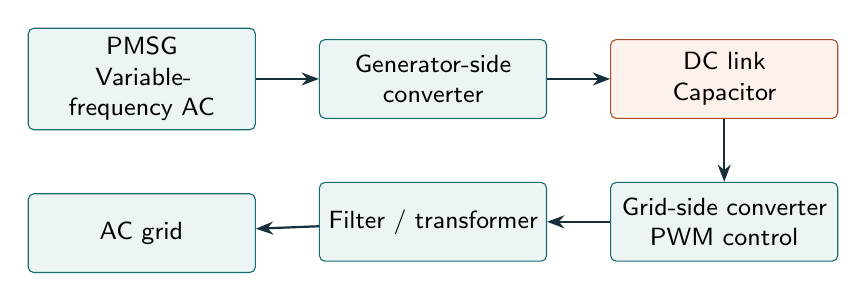
\begin{tikzpicture}[node distance=8mm and 8mm]
\node[block] (g) {PMSG\\Variable-frequency AC};
\node[block,right=of g] (gc) {Generator-side\\converter};
\node[hot,right=of gc] (dc) {DC link\\Capacitor};
\node[block,below=of dc] (inv) {Grid-side converter\\PWM control};
\node[block,below=of gc] (f) {Filter / transformer};
\node[block,below=of g] (grid) {AC grid};
\draw[arr] (g)--(gc);\draw[arr] (gc)--(dc);\draw[arr] (dc)--(inv);\draw[arr] (inv)--(f);\draw[arr] (f)--(grid);
\end{tikzpicture}
\end{center}
Rotor speed can vary to capture wind energy, so generator frequency varies. The DC link decouples the generator-side electrical frequency from grid frequency. The grid-side converter injects controlled AC current; voltage / current sensing and DC-link measurement support its controller. \textbf{PWM} means pulse-width modulation. The capacitor supports short-term converter energy balance; it is not a bulk multi-hour storage battery.

A doubly-fed induction generator (DFIG) uses a different connection with a converter in the rotor circuit; not all wind turbines send all generator power through the particular full-converter path above. For this module, explain the supplied PMSG schematic without assuming it is universal.

\subsection{Types: horizontal / vertical, onshore / offshore}
A \textbf{horizontal-axis turbine} rotates about an approximately horizontal axis, commonly with three blades and a yaw mechanism. A \textbf{vertical-axis turbine} rotates about a vertical axis; many designs accept wind from different directions without yawing. Darrieus designs use lift; Savonius designs primarily use drag. The side-by-side class image distinguishes axes, not just different blade appearance.

\textbf{Onshore} projects generally have easier access / construction. \textbf{Offshore} projects can access strong winds and larger turbines, but require marine foundations / structures, subsea cables, corrosion control and difficult maintenance. The offshore photograph in p. 74 illustrates these added site constraints. Stronger wind does not make every offshore project have the same capacity factor.

\subsection{Cut-in, rated and cut-out: why cubic scaling has limits}
Below \textbf{cut-in speed}, generation is absent or impractical. From cut-in toward rated speed, available power rises strongly. Near / above \textbf{rated speed}, pitch / control limits output to the machine rating. At unsafe \textbf{cut-out conditions}, the turbine shuts down or enters its designed high-wind strategy to protect equipment. Thus doubling wind speed does not always produce eight times electrical power, even though available wind power scales as $v^3$ in the simple relation.

\subsection{Advantages, disadvantages and environmental factors}
\textbf{Advantages:} renewable resource; no fuel consumption for normal output; low operational emissions; relatively low water use; farming can continue between turbines; onshore / offshore and distributed deployment options.

\textbf{Disadvantages:} variable wind and forecasting error; suitable sites / transmission required; mechanical maintenance; access difficulties offshore; visual / acoustic impacts and potential bird / bat collisions. Spacing reduces wakes, so a farm occupies an area wider than the actual turbine foundations.

Environmental assessment should consider bird / bat migration / habitats, noise, shadow flicker, landscape and community concerns. Offshore projects also need marine ecological and shipping / fishing assessment. Careful siting, wildlife monitoring, targeted curtailment and appropriate setbacks reduce impacts. Lifecycle material extraction and blade / material recycling matter even when the turbine does not burn fuel. Noise concerns should be measured and addressed, rather than converted into an unsupported blanket health claim.

\subsection{Notable project examples}
Muppandal, Kanyakumari / Tamil Nadu (about 1500 MW in the slides), illustrates use of strong Western Ghats / pass winds. Gansu, China, is quoted with a \textbf{planned} 20000 MW figure. Planned, installed and currently available capacities are different. Regulations and ecological permissions are explained next.
\checkq{What is the difference between pitch and yaw?}{Pitch rotates a blade around its own axis to adjust aerodynamic action; yaw turns the nacelle / rotor direction around the tower to face the wind.}

\chapterstart{Renewable regulations and the wider transition}{policy}
\slides{Part 1 pp. 53, 56, 68, 78--79, 90--93}
\subsection{What a regulation answer should accomplish}
Regulation both \textbf{promotes renewable deployment} and \textbf{sets conditions for safe, fair operation}. An answer listing only subsidies misses grid, land, ecological and consumer-protection requirements. Describe the mechanism, its purpose and the engineering connection. The following explains the class examples; detailed eligibility, quotas, tariffs and local permissions must use the applicable dated notification.

\subsection{Indian renewable policy framework}
\begin{enumerate}
\item \textbf{National Solar Mission (2010):} the class identifies a national programme to promote solar deployment, reduce costs and develop the sector. Its role is market / technology development, rather than a power-conversion device. See MNRE's official material [R1].
\item \textbf{Renewable Purchase Obligation (RPO):} specified obligated entities must meet applicable renewable procurement requirements. Obligations and compliance categories vary with the current framework and entity; they should not be assumed identical for every consumer. Renewable energy certificates are a related compliance mechanism under CERC rules [R3]. An RPO is a procurement requirement, not a guaranteed payment to a producer.
\item \textbf{PM Surya Ghar: Muft Bijli Yojana (2024):} supports household rooftop-solar adoption through financial assistance and implementation arrangements. System design, actual generation, consumption and applicable metering rules determine the electricity / bill outcome. The programme name is not a technical guarantee that every household receives identical energy each month. Refer to official scheme guidelines [R1].
\item \textbf{National Wind-Solar Hybrid Policy (2018):} promotes integrated wind / PV projects, better use of land and transmission, and reduced aggregate variability. Sharing infrastructure can improve utilisation because outputs need not peak together. Hybrid generation still needs resource assessment, dispatch and connection design; it does not automatically give constant output. Official policy context is confirmed by the 2018 MNRE / PIB announcement [R2].
\item \textbf{500 GW by 2030:} the target quoted is \textbf{installed non-fossil electricity capacity}, not 500 GW of continuous output or 500 GWh of energy. Non-fossil includes nuclear, whereas renewable and non-fossil are not identical categories. Official context: PIB [R10].
\end{enumerate}

\begin{Caution}{Date-sensitive material}
Official policy pages were checked on 8 October 2026. This is a conceptual study summary, not an exhaustive statement of current law. The slide years identify when initiatives began. Numerical quotas, subsidies, net-metering limits and project clearances can change; no obsolete percentage or subsidy amount is required for the Module 1 definitions.
\end{Caution}

\subsection{Global mechanisms: distinguish their functions}
\begin{center}\small
\begin{tabularx}{\textwidth}{L{3.3cm}YY}
\toprule\textbf{Mechanism} & \textbf{What it does} & \textbf{Why it affects generation}\\\midrule
RPS / renewable quotas & Requires a specified renewable share from obligated suppliers / entities under that jurisdiction & Creates demand for renewable output\\
Feed-in tariff (FIT) & Pays eligible renewable producers a defined tariff under a scheme & Gives revenue certainty and encourages investment\\
Competitive auction & Developers bid for a defined procurement requirement & Competition can lower offered prices, subject to delivery and contract conditions\\
Net metering & Measures imports / exports and credits them under local rules & Supports rooftop self-generation and permitted surplus export\\
Carbon tax & Charges for eligible emissions under the scheme & Reflects part of pollution cost in decisions\\
Emissions trading (ETS) & Uses tradable allowances under a cap / design & Creates an emissions-price incentive\\\bottomrule
\end{tabularx}\end{center}
\textbf{Net and gross metering differ:} net metering accounts for imported / exported energy under its settlement rules; gross metering separately accounts for generation supplied and consumption purchased. Credits are not necessarily equal to cash at the retail tariff. RPO / RPS, FIT, net metering and carbon pricing should not be used as synonyms.

\subsection{Practical permissions and grid conditions}
\begin{itemize}
\item \textbf{Solar:} land / roof rights, structural adequacy, suitable ecological / planning permissions, electrical protection, approved metering and grid connection. An anti-islanding requirement protects people and equipment when the utility supply fails.
\item \textbf{Wind:} siting and setbacks where applicable, noise / shadow assessment, wildlife surveys, aviation / obstacle issues and network connection. Offshore development also considers marine ecology, shipping lanes and seabed / coastal permissions.
\item \textbf{Both:} forecasting / scheduling where required, power quality, voltage / reactive-power capabilities and relevant grid-code compliance. The exact obligations depend on voltage, plant size, jurisdiction and the dated code.
\end{itemize}
Carbon pricing / quota policies address markets; grid codes address electrical behaviour; permits address sites and impacts. Good regulation must address all three.

\subsection{Environmental justice and system design}
The class's energy transition discussion includes material supply chains, land conflicts and fair sharing of costs. Batteries can require lithium / nickel / cobalt depending on chemistry; some wind generators use rare-earth magnets, while other designs do not. Avoid assuming every battery contains cobalt or every wind turbine requires rare-earth magnets.

Responsible sourcing, recycling, community participation and worker protection matter alongside decarbonisation. Agrivoltaics, rooftops and suitable floating solar can reduce some land conflicts; offshore deployment brings different ecological / maintenance burdens. Network expansion moves renewable power from resource regions to loads. Storage, forecasting, geographically diverse sources and demand response address variability together.

\subsection{Generation economics and future horizons}
\textbf{Levelised cost of energy (LCOE)} spreads lifetime plant cost over discounted lifetime energy. Low generation LCOE alone does not describe full system cost, which also includes firm capacity, flexibility, transmission and integration. Slide claims about percentage cost falls, investment rankings or a particular future year are contextual trend statements, not constants to memorise.

\textbf{Externalities} are costs imposed on others, such as pollution damage. Carbon pricing aims to \emph{internalise} some of those costs in market decisions. \textbf{Green hydrogen} uses renewable electricity for electrolysis, stores chemical energy and can supply industry or later energy conversion; conversion losses and infrastructure matter. \textbf{Fusion} combines light nuclei and remains a development / research topic; a commercial arrival year is uncertain. Fission is the nuclear generation method studied in this module.
\checkq{Why might a wind-solar hybrid improve infrastructure use?}{If wind and PV peak at different times, shared land / network infrastructure can be used more evenly. The extent of benefit depends on the actual resource profiles.}

\chapterstart{Energy storage: BESS, CESS and thermal systems}{storage}
\slides{Part 1 pp. 81--88; supporting context pp. 89--93}
\subsection{Storage as an alternative source of supply}
Storage \textbf{absorbs energy earlier} and \textbf{supplies it later}. During discharge it is an alternative source at the point of use, but it is not an independent primary energy source. Storage loses energy through conversion and self-discharge / heat leakage.

The slides use \textbf{CESS} for compressed-air / energy storage; \textbf{CAES} is the common acronym for compressed-air energy storage. \textbf{Thermal SS}, \textbf{TES} and \textbf{TESS} here all refer to thermal energy storage systems. Keep the class label while stating the mechanism unambiguously.

\subsection{Why the grid uses storage}
\begin{itemize}
\item \textbf{Energy shifting:} charge during renewable surplus / low demand, discharge later.
\item \textbf{Peak shaving:} reduce the maximum import or required generation during a short peak.
\item \textbf{Renewable firming / smoothing:} buffer changes within the available power / energy limits.
\item \textbf{Frequency support:} alter active power rapidly when suitably controlled and charged.
\item \textbf{Backup / restoration:} supply important loads or assist black start when designed for that service.
\item \textbf{Reduced curtailment:} capture energy that cannot otherwise be used / exported at that time.
\end{itemize}
A solar-rich grid may have low net demand at midday and a steep evening rise as PV declines, often called the \textbf{duck curve}. Storage and flexible loads can move some midday energy use and reduce the evening ramp. Adequate transmission / interconnection, dispatchable resources and demand response also matter; one MW of renewable capacity does not inherently require exactly one MW of conventional backup.

\subsection{Power rating, energy rating and losses}
\begin{Idea}{MW answers ``how fast?''; MWh answers ``how long?''}
A usable $20\,\mathrm{MW}/80\,\mathrm{MWh}$ store can ideally deliver 20 MW for 4 h. It can deliver only 10 MW for 8 h if operational constraints allow. It cannot deliver 40 MW merely because 80 MWh is available: the power-conversion equipment sets the power limit.
\[
t_{\rm discharge}=\frac{E_{\rm usable}}{P_{\rm discharge}},\qquad
\eta_{\rm rt}=\frac{E_{\rm electrical,out}}{E_{\rm electrical,in}}.
\]
Use comparable measurement boundaries and a full charge / discharge cycle for round-trip efficiency.
\end{Idea}
If a system returns 90 MWh for 100 MWh supplied during charging, round-trip efficiency is 90\%. A nameplate energy rating may not equal usable AC output: state-of-charge limits, degradation, discharge losses and reserved energy reduce available delivery. Do not apply an efficiency twice if a problem already gives usable delivered energy.

\subsection{BESS: the battery is only one part of the system}
\begin{center}
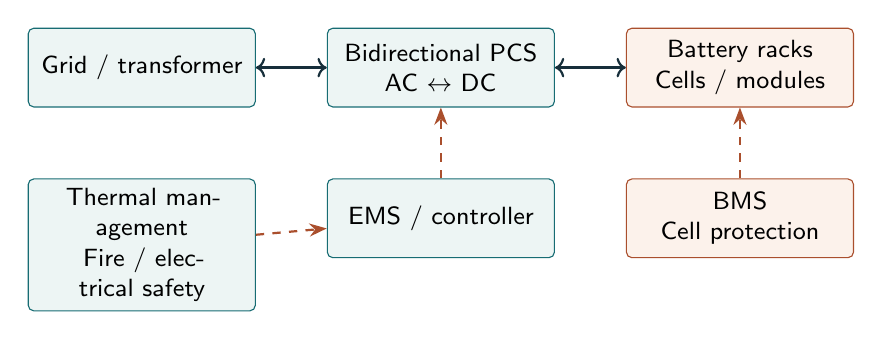
\begin{tikzpicture}[node distance=9mm and 9mm]
\node[block] (grid) {Grid / transformer};
\node[block,right=of grid] (pcs) {Bidirectional PCS\\AC $\leftrightarrow$ DC};
\node[hot,right=of pcs] (bat) {Battery racks\\Cells / modules};
\node[hot,below=of bat] (bms) {BMS\\Cell protection};
\node[block,below=of pcs] (ems) {EMS / controller};
\node[block,below=of grid] (safe) {Thermal management\\Fire / electrical safety};
\draw[arr,<->] (grid)--(pcs);\draw[arr,<->] (pcs)--(bat);
\draw[control] (bms)--(bat);\draw[control] (ems)--(pcs);\draw[control] (safe)--(ems);
\end{tikzpicture}
\end{center}
\diagramcaption{PCS = power conversion system, BMS = battery management system, EMS = energy management system. Dashed connections indicate supervision / control; safety equipment also acts directly on the physical system.}

\subsubsection{Charging and discharging}
During \textbf{charge}, electrical input drives electrochemical changes that store energy. During \textbf{discharge}, the reactions supply DC electrical power; the PCS converts it to AC for the grid. This is not merely ``storing AC inside a box.''

\begin{itemize}
\item \textbf{Cells / modules / racks:} create the voltage and energy capacity.
\item \textbf{BMS:} monitors cell voltage, temperature and state of charge, balances cells, and protects against overcharge / overdischarge or unsafe operation.
\item \textbf{PCS:} sets charging / discharging power within current / voltage limits, converts AC / DC, and supports assigned grid functions.
\item \textbf{EMS:} schedules operation using demand, resource, tariffs and constraints. A fast converter cannot discharge an empty battery.
\item \textbf{Cooling, ventilation, detection and isolation:} manage heat and fire / electrical risks. Cooling can be air- or liquid-based; no cooling method guarantees that thermal runaway can never occur.
\end{itemize}

\subsubsection{Chemistries and class examples}
The slides highlight lithium-ion \textbf{NMC} (nickel manganese cobalt) and \textbf{LFP} (lithium iron phosphate). Chemistry affects energy density, cycle life, cost and safety. LFP avoids cobalt in its cathode and generally has favourable thermal stability; it still requires suitable protection. Flow batteries separate stored electrolyte energy capacity from stack power more directly than conventional packaged cells. Solid-state batteries are a development direction, not a necessary assumption for present BESS operation.

The class gives \textbf{Hornsdale Power Reserve, Australia} as a project and \textbf{Tesla Megapack} as a product example. These are distinct examples; do not assume a named product is necessarily the equipment used in that project.

\subsubsection{Advantages and disadvantages}
\textbf{Advantages:} fast response, modular siting, high electrical round-trip efficiency, reversible power flow and useful renewable / peak / frequency services. The class quotes 85--95\% efficiency and common 1--4 h durations as illustrative Li-ion figures; real design values vary and duration is not a fundamental battery limit.

\textbf{Disadvantages:} degradation with age / cycling, finite energy, replacement cost, temperature sensitivity, fire / electrical risks, mining / manufacturing impacts and recycling needs. Synthetic inertia or grid-forming support requires appropriate controls and headroom; it is not an automatic property of every battery installation.

\subsection{CESS / CAES: compressed-air storage}
\begin{center}
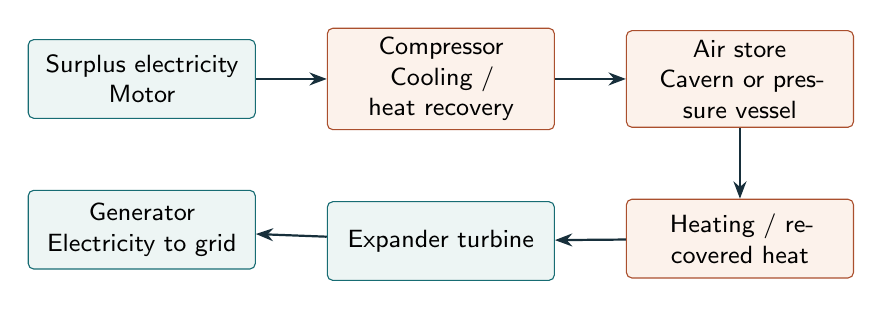
\begin{tikzpicture}[node distance=9mm and 9mm]
\node[block] (grid) {Surplus electricity\\Motor};
\node[hot,right=of grid] (comp) {Compressor\\Cooling / heat recovery};
\node[hot,right=of comp] (store) {Air store\\Cavern or pressure vessel};
\node[hot,below=of store] (heat) {Heating / recovered heat};
\node[block,below=of comp] (exp) {Expander turbine};
\node[block,below=of grid] (gen) {Generator\\Electricity to grid};
\draw[arr] (grid)--(comp);\draw[arr] (comp)--(store);\draw[arr] (store)--(heat);\draw[arr] (heat)--(exp);\draw[arr] (exp)--(gen);
\end{tikzpicture}
\end{center}
\diagramcaption{Charge path is across the top; discharge path is along the lower row. Heat handling is essential to interpreting compressed-air storage.}
\begin{enumerate}
\item During charge, electricity drives compressors. Air becomes hotter during compression.
\item Air is stored under pressure in a suitable sealed cavern or pressure vessel.
\item During discharge, air is conditioned / heated and expanded through a turbine driving a generator. Expansion cools air; maintaining useful inlet conditions improves output and avoids operating problems.
\end{enumerate}

\subsubsection{Diabatic and adiabatic designs}
\textbf{Conventional diabatic CAES} rejects much of compression heat and commonly adds fuel heat during discharge. It is therefore not necessarily emission-free. \textbf{Adiabatic CAES} retains compression heat in a thermal store and uses it during discharge, reducing / eliminating the need for that fuel heat depending on the design. Near-isothermal approaches seek to manage temperature changes during compression / expansion. Sandia's storage material provides supporting context [R7].

\textbf{Advantages:} potential bulk / multi-hour storage, long-lived mechanical assets and a useful complement to variable generation. \textbf{Disadvantages:} site / geology constraints for cavern systems, pressure-vessel / cavern integrity requirements, heat-management complexity, mechanical losses and potentially fuel / emissions. Tanks offer alternatives at other scales but do not remove all cost / safety constraints.

The class quotes hundreds of MWh and 40--70\% round-trip efficiency as illustrative values. For fuel-assisted systems, efficiency comparisons depend on whether / how fuel input is counted. Do not rank CAES against a battery using inconsistent energy boundaries. Suitable geology must be demonstrated; any abandoned mine or aquifer cannot simply be assumed safe for compressed air.

\subsection{Thermal storage: retain useful heat or cold}
Thermal storage holds energy in a medium for later electricity production, heating or cooling. The delivered product matters: stored heat used directly is different from heat converted back to electricity through a heat engine.

\begin{center}\small
\begin{tabularx}{\textwidth}{L{3cm}YY}
\toprule\textbf{Type} & \textbf{How energy is retained} & \textbf{Examples}\\\midrule
Sensible heat & Temperature of a material changes & Hot water, molten salt, rock beds\\
Latent heat & A phase change stores / releases energy & Ice, other phase-change materials\\
Thermochemical (extension) & Reversible chemical processes & Specialised / developing heat-storage systems\\\bottomrule
\end{tabularx}\end{center}
For sensible heat, $E_{\rm th}\approx m c_p\Delta T$ if heat capacity is treated as constant. For a phase change, $E_{\rm latent}=mL$ for the idealised transition. These optional relations explain why both a temperature rise and melting / freezing can store energy.

\subsubsection{Two-tank molten-salt storage with CSP}
Cold-tank salt is heated through the solar receiver and sent to the hot tank. When electricity is needed, hot salt transfers heat in a steam generator and returns to the cold tank. The steam turbine produces shaft work / electricity. Salt and steam normally remain separate fluids.
\begin{center}
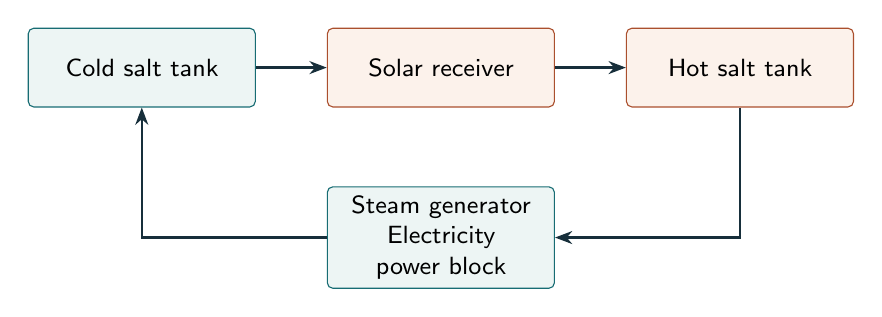
\begin{tikzpicture}[node distance=10mm and 9mm]
\node[block] (cold) {Cold salt tank};
\node[hot,right=of cold] (rec) {Solar receiver};
\node[hot,right=of rec] (hot) {Hot salt tank};
\node[block,below=of rec] (hx) {Steam generator\\Electricity power block};
\draw[arr] (cold)--(rec);\draw[arr] (rec)--(hot);\draw[arr] (hot.south)|-(hx.east);\draw[arr] (hx.west)-|(cold.south);
\end{tikzpicture}
\end{center}
Other heat stores use stratified tanks / rock beds rather than exactly two tanks. The insulated store cutaway in Part 1 p. 87 illustrates a contained medium, heat exchange / flow paths, structural shell and insulation. Insulation slows losses; it does not eliminate them.

\subsubsection{Cold storage and useful applications}
An ice / chilled-water system makes cold during an earlier period and uses it for cooling during a peak. This can shift air-conditioning electricity demand without generating electrical output. Other uses include industrial process heat and district heating. CSP heat storage makes evening generation possible within the stored heat and power-block limits.

\textbf{Advantages:} useful for matching heat / cooling demand, low-cost bulk media in suitable applications, reduced peak demand and better use of solar / waste heat. \textbf{Disadvantages:} thermal losses, volume / insulation requirements, material compatibility / corrosion, molten-salt freezing risks, pumping and heat-exchanger limits. Heat-to-electricity conversion introduces additional losses.

\begin{Caution}{Thermal efficiency is not one universal percentage}
A store's retained heat fraction, heat delivered for heating, and electricity-to-electricity round-trip efficiency are different quantities. A thermal store can deliver heat efficiently while its electricity recovery is much lower because of the heat engine. The old shortcut of assigning one generic TES efficiency cannot describe all these services.
\end{Caution}

\subsection{Choose storage by the service required}
The comparison in Section~\ref{storagecomparison} collects the stored forms, services and constraints for revision.
Choose power, useful duration, response, cycling, efficiency boundaries, lifetime, site, emissions and cost together. Longer duration is useful only when there is enough charging energy and the service needs it.
\checkq{Does a 100 MWh battery necessarily cover a 100 MW peak for one hour?}{Only if at least 100 MWh is usable at the delivery boundary and its power rating / operating constraints permit 100 MW. Nameplate MWh alone is insufficient.}

\chapterstart{Load curves and generation scheduling}{curves}
\slides{Part 2 pp. 2--9, 21--29}
\subsection{Demand is measured at a defined boundary}
A load curve may describe a consumer, feeder, region or entire station. Decide \textbf{which boundary} and \textbf{which period} the data refer to. Consumer energy and generated energy differ by network losses and auxiliary consumption. Class numerical problems usually neglect these differences unless stated.

Demand can change with time of day, weekday, season, weather and industrial / domestic behaviour. Metered maximum demand is commonly an average over a specified interval (the slides illustrate 15/30 min), rather than a millisecond current surge. In a piecewise-constant class problem, the highest listed load is the maximum demand.

\subsection{Chronological load curve}
A \textbf{load curve} plots power demand vertically against chronological time horizontally. A daily curve spans 24 h; a yearly curve spans the stated year. Its highest point gives maximum demand; its area gives energy:
\[
E=\int_0^T P(t)\,dt,\qquad E=\sum_i P_i\Delta t_i\quad\text{for blocks}.
\]
The average load is the height of a rectangle covering the same time and area:
\[
P_{\rm av}=\frac{E}{T}.
\]
It is a \textbf{time-weighted} average. An arithmetic average of load levels works only when their durations are equal.

\subsection{Constructing the load-duration curve}
\begin{enumerate}
\item Read every chronological load block and its duration.
\item Sort blocks by power in descending order; keep each block's duration attached.
\item Put the largest load first, then accumulate durations left to right.
\item Label the horizontal axis \textbf{duration}, not clock time.
\end{enumerate}
For hourly samples, each sample has width 1 h. For unequal blocks, the widths remain unequal. At a chosen load threshold, the horizontal extent indicates the total duration for which demand is at least that level (step endpoints have no effect on energy).

\begin{center}
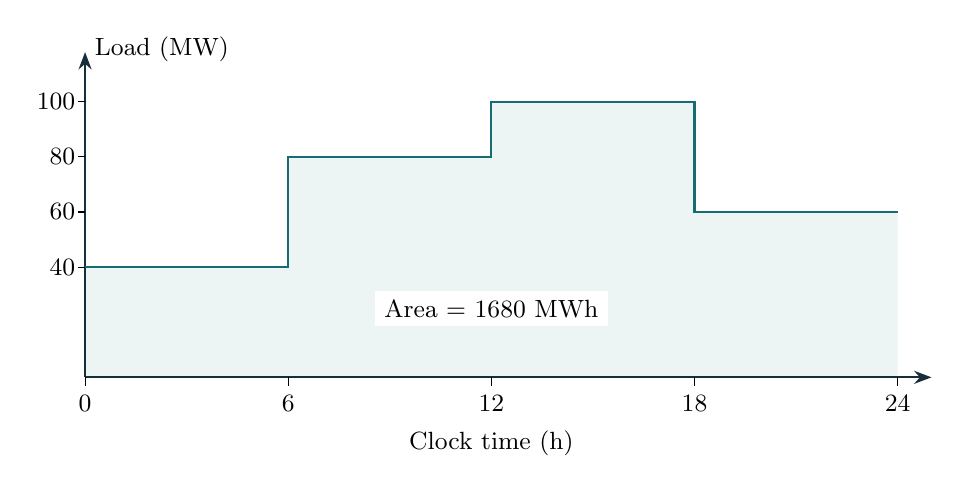
\begin{tikzpicture}[x=.43cm,y=.035cm]
\fill[pale] (0,0)--(0,40)--(6,40)--(6,80)--(12,80)--(12,100)--(18,100)--(18,60)--(24,60)--(24,0)--cycle;
\draw[arr] (0,0)--(25,0);\draw[arr] (0,0)--(0,118);
\draw[thick,teal] (0,40)--(6,40)--(6,80)--(12,80)--(12,100)--(18,100)--(18,60)--(24,60);
\foreach \x in {0,6,12,18,24}{\draw (\x,0)--(\x,-3) node[below,font=\small]{\x};}
\foreach \y in {40,60,80,100}{\draw (-.2,\y)--(0,\y) node[left,font=\small]{\y};}
\node[font=\small] at (12,-24) {Clock time (h)};
\node[font=\small,anchor=west] at (0,119) {Load (MW)};
\node[font=\small,fill=white] at (12,25) {Area = 1680 MWh};
\end{tikzpicture}
\end{center}
\diagramcaption{Daily class schedule: 40 MW for 6 h, then 80 MW, 100 MW and 60 MW for 6 h each. Chronology shows when the noon peak occurs.}

\begin{center}
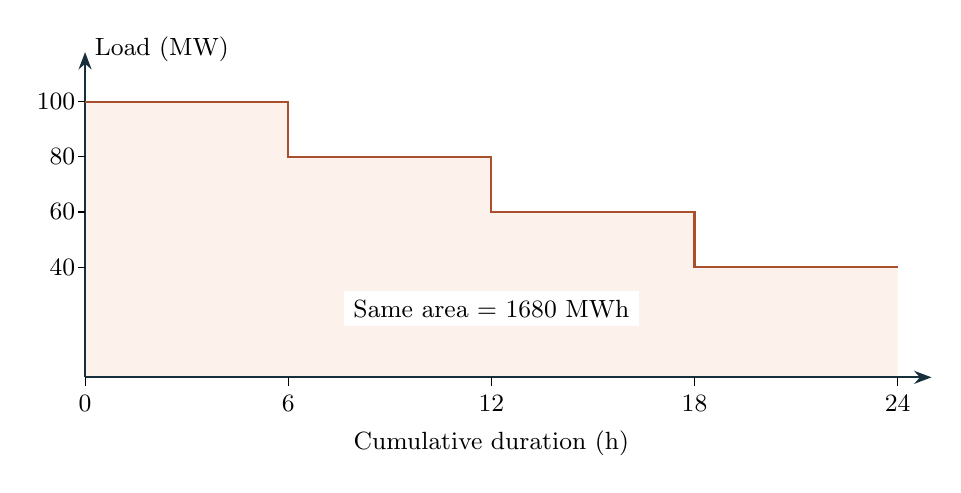
\begin{tikzpicture}[x=.43cm,y=.035cm]
\fill[warm] (0,0)--(0,100)--(6,100)--(6,80)--(12,80)--(12,60)--(18,60)--(18,40)--(24,40)--(24,0)--cycle;
\draw[arr] (0,0)--(25,0);\draw[arr] (0,0)--(0,118);
\draw[thick,rust] (0,100)--(6,100)--(6,80)--(12,80)--(12,60)--(18,60)--(18,40)--(24,40);
\foreach \x in {0,6,12,18,24}{\draw (\x,0)--(\x,-3) node[below,font=\small]{\x};}
\foreach \y in {40,60,80,100}{\draw (-.2,\y)--(0,\y) node[left,font=\small]{\y};}
\node[font=\small] at (12,-24) {Cumulative duration (h)};
\node[font=\small,anchor=west] at (0,119) {Load (MW)};
\node[font=\small,fill=white] at (12,25) {Same area = 1680 MWh};
\end{tikzpicture}
\end{center}
\diagramcaption{Corresponding LDC: 100, 80, 60 and 40 MW, each for 6 h. The first 6 h means the six highest-demand hours, not necessarily midnight to 6 a.m.}

\subsection{What sorting preserves, and what it loses}
\begin{center}\small
\begin{tabularx}{\textwidth}{L{3.5cm}YY}
\toprule\textbf{Information} & \textbf{Load curve} & \textbf{LDC}\\\midrule
Energy, maximum / minimum, average & Available & Preserved\\
Duration above a threshold & Can be counted & Directly visible\\
Time at which a peak occurs & Available & Lost\\
Ramps, consecutive peaks, order & Available & Lost\\
Detailed start / stop / storage scheduling & Requires chronological data & Insufficient alone\\\bottomrule
\end{tabularx}\end{center}
Sorting does not change $\sum P_i\Delta t_i$. Hence the area, average load and load factor are the same. Two very different chronological profiles can have the same LDC. One may need hours of consecutive discharge while the other has intervening opportunities to charge. \textbf{Do not size storage from the LDC alone.}

\subsection{Base, intermediate and peak loads}
\textbf{Base load} is the part of demand present throughout the period (the minimum of the curve in a simple model). \textbf{Intermediate load} lies above it for substantial portions of the period. \textbf{Peak load} occurs briefly at the top.

These are demand categories, not immutable labels attached to fuels. In the traditional plant mix, low-variable-cost units with high fixed cost often meet sustained demand; flexible units meet shorter peaks. Reservoir hydro, pumped storage, batteries and simple-cycle gas turbines can provide peak / flexibility services. Combined-cycle units often follow intermediate demand. PV can lower midday net load, changing which conventional units are needed.

A \textbf{base plant} with capacity $P_b$ can supply at most the actual demand, if export / storage is absent. Its ideal scheduled output is
\[
P_{b,\rm out}(t)=\min\{P_b,P(t)\}.
\]
It is wrong to assign it $P_bT$ energy if load drops below $P_b$. Example~\ref{ldcexample} develops this point.

\subsection{Plant scheduling, reserve and costs}
A chronological load curve helps schedule units, estimate ramps, plan maintenance and forecast expansion. An LDC helps understand how often different capacities will be used. Detailed economic dispatch additionally needs cost curves, unit limits, reserves and network constraints.

\textbf{Spinning reserve} is additional output available from online synchronised plant within the required response time; an online unit can be partly loaded and hold headroom. It need not be fully unloaded. Other response services can come from batteries, demand response and qualified offline resources.

Frequent steam-plant cycling causes temperature / stress cycles in boiler / turbine parts and may increase maintenance. At part load, heat rate (fuel heat per electrical kWh) commonly rises. The slides' 15--25\% figure illustrates possible penalties, not a universal constant. Reliable capacity can be costly while idle, but too little capacity creates supply risk.

\subsection{Demand-side management and forecasting}
\textbf{Peak shifting} moves flexible consumption to off-peak periods; \textbf{peak shaving} reduces peak power; \textbf{valley filling} adds suitable demand at low-load times. Examples are scheduled EV charging, industrial process timing and chilled-water storage. Reducing peak while preserving useful energy generally improves load factor.

Smart meters and two-way communication enable demand response. Weather / history-driven forecasting helps anticipate load and renewable output. Automated / AI-assisted control still needs measurements, constraints, adequate reserves and sound engineering; it cannot create physical capacity. The class's ``human factor'' is that demand curves record actual patterns of people's activity, so planning serves users as well as machines.
\checkq{If an LDC shows 80 MW for 12 h, do those hours necessarily occur consecutively?}{No. They are the cumulative duration at or above that load. Sorting removed their clock-time order.}

\chapterstart{Load and plant factors}{factors}
\slides{Part 2 pp. 11--18, 24}
\subsection{Notation and a consistent time basis}
\begin{center}\small
\begin{tabularx}{\textwidth}{L{2.5cm}Y L{2.5cm}}
\toprule\textbf{Symbol} & \textbf{Meaning} & \textbf{Unit}\\\midrule
$C$ & Connected load: sum of relevant ratings of connected equipment & kW or MW\\
$M$ & Maximum demand during the stated period & kW or MW\\
$P_c$ & Installed / rated plant capacity & kW or MW\\
$E$ & Actual energy generated / supplied in that period & kWh or MWh\\
$T$ & Total elapsed period, including downtime & h\\
$T_o$ & Time the stated plant is actually operating & h\\
$P_{\rm av}$ & Average over the full period, $E / T$ & kW or MW\\\bottomrule
\end{tabularx}\end{center}
For the simplified problems, take ratings constant and demand / output at a common boundary, neglecting losses unless given. A real multi-unit station may require a carefully defined operating-time benchmark; use the definition supplied in the problem.

\subsection{Demand factor: how much connected load is demanded?}
\[
\boxed{DF=\frac{M}{C}}\qquad M=DF\,C.
\]
A site may have 500 kW of connected equipment but a recorded peak of only 350 kW, because equipment is not all on at full demand simultaneously. Then $DF=0.70$. It compares \textbf{the peak to an equipment-rating total}; it does not compare average and peak.

Usually $0\le DF\le1$ under the textbook assumptions. \textbf{Equality is possible}: all rated connected equipment may be used together. An abnormal overload or inconsistent power-rating basis is outside the simple rule. A low demand factor does not itself create spare generator capacity; it describes how consumer equipment is used.

\subsection{Diversity factor: individual peaks versus combined peak}
\[
\boxed{DivF=\frac{\sum_i M_i}{M_{\rm system}}}\qquad
M_{\rm system}=\frac{\sum_i M_i}{DivF}.
\]
Each consumer's maximum may occur at a different time. The system maximum is the maximum of their \textbf{simultaneous sum}, not the sum of their separate maxima:
\[
\max_t\left(\sum_iP_i(t)\right)\le\sum_i\max_t P_i(t).
\]
Therefore $DivF\ge1$ for positive normal loads on a consistent period. \textbf{Equality is possible} if all peaks coincide. Higher diversity can reduce required feeder / transformer / plant power compared with adding all individual peaks.

The \textbf{coincidence factor} is the reciprocal, $CF_{\rm coincidence}=1/DivF$, and is at most 1. It is distinct from plant capacity factor; avoid using the same abbreviation ambiguously.

\begin{Worked}{A time-based explanation of diversity}
Consumer A uses 40 kW in the morning and 10 kW in the evening. Consumer B uses 10 kW in the morning and 60 kW in the evening. Individual peaks sum to $40+60=100$ kW, while simultaneous totals are 50 kW and 70 kW.\par
Thus $M_{\rm system}=70$ kW and $DivF=100/70=1.429$. Using 100 kW as the combined maximum would throw away the non-coincidence of their peaks.
\end{Worked}

\subsection{Load factor: how steady is the load?}
\[
\boxed{LF=\frac{P_{\rm av}}{M}=\frac{E}{M T}}\qquad E=LF\,M T.
\]
A rectangle of height $M$ lasting $T$ would have energy $MT$. Load factor is the actual curve area divided by that rectangle's area. $LF=1$ means constant load at its maximum throughout the period. Lower values mean the average is lower relative to the peak.

A high load factor usually spreads fixed supply costs over more kWh, for the same required peak capacity. It is a utilisation statistic, not fuel-to-electricity efficiency. Improving it can mean reducing peak while preserving energy, or increasing useful off-peak demand. No single ``good'' value applies to every consumer / plant type.

\subsection{Plant capacity factor: compare with continuous rated output}
\[
\boxed{PCF=\frac{E}{P_c T}=\frac{P_{\rm av}}{P_c}}.
\]
The denominator assumes the plant runs at installed capacity throughout \emph{all} elapsed hours. Outages, part loading, resource variability and deliberate non-dispatch lower this factor. If a 100 MW plant generates 1440 MWh in 24 h, its capacity factor is $1440/2400=0.60$.

\textbf{Load factor's denominator is peak demand; capacity factor's is rated plant capacity.} They are equal only if $M=P_c$ on the same basis. A 100 MW plant averaging 50 MW with a peak of 80 MW has $LF=62.5\%$ but $PCF=50\%$.

\subsection{Plant use factor: compare with rated output while operating}
\[
\boxed{PUF=\frac{E}{P_c T_o}}.
\]
The denominator ignores hours when the stated plant is not operating. For a 120 MW plant generating 1440 MWh over 16 operating hours within a 24 h day, $PUF=75\%$, whereas $PCF=50\%$.

Its average output \textbf{while operating} is $E / T_o=90$ MW. The average over \textbf{the whole day} is $E / T=60$ MW. Plant use factor measures loading during operation; it does not measure the ratio of electrical output to fuel input.

\subsection{Derive useful relationships instead of memorising blindly}
Let the supporting \textbf{utilisation factor} be $UF=M / P_c$. Then
\begin{align*}
PCF&=\frac{E}{P_c T}
=\left(\frac{E}{M T}\right)\left(\frac{M}{P_c}\right)
=LF\,UF,\\
PCF&=\left(\frac{E}{P_c T_o}\right)\left(\frac{T_o}{T}\right)
=PUF\,\frac{T_o}{T}.
\end{align*}
Thus $T_o=T(PCF / PUF)$ for positive factors; use fractions consistently. The ratio $T_o / T$ is operating-time fraction, not necessarily technical availability (a technically available plant can be deliberately idle).

The class-style \textbf{reserve capacity} is $P_c-M$. This is an arithmetic capacity margin; it does not prove the reserve is online, dependable or sufficient after an outage. Variable-resource nameplate capacity cannot automatically be counted as firm reserve.

\begin{Idea}{Consistency checks for ordinary class problems}
With positive demand and $M\le P_c$:
\[
0<LF\le1,\quad 0<DF\le1,\quad DivF\ge1,
\quad PCF\le LF,\quad PCF\le PUF\le1.
\]
Also $P_{\rm av}\le M$, $E\le MT$, $E\le P_cT_o$ and $T_o\le T$. A ratio outside the expected bounds often signals a wrong unit, denominator or inconsistent dataset. Some ratios are undefined for a completely zero-load / no-operation period, so do not divide by zero.
\end{Idea}

\subsection{A denominator-first method for numerical problems}
\begin{enumerate}
\item Write the known values $C,M,P_c,E,T,T_o$; leave unknowns blank.
\item Convert energy and power to compatible prefixes.
\item Calculate $P_{\rm av}=E / T$ using the full period.
\item Select the denominator by meaning: $C$, $M$, $P_cT$ or $P_cT_o$.
\item For diversity, determine individual maximum demands first, then divide their sum by the system peak (or solve the inverse).
\item Check bounds and use the two relationships above.
\end{enumerate}
\checkq{If a plant is idle for half a day, should the daily average load use 12 h or 24 h?}{Use 24 h for daily average and capacity / load factors. Use 12 operating hours only for the plant-use benchmark or operating-hours average.}

\chapterstart{Every class numerical, fully worked}{classproblems}
The three introductory examples and seven numbered end-of-deck problems are all included below. Slide-page anchors let you match each solution to class. Symbols follow Section~\ref{factors}; percentages are rounded only at the final step.

\subsection{Class example 1: residential feeder and diversity}
\slides{Part 2 p. 19}
\begin{Worked}{Given and required}
Three groups have connected loads 2500, 1800 and 1200 kW, with demand factors 0.50, 0.60 and 0.55 respectively. The group counts in the slide are 50, 30 and 20 homes. Diversity factor for the combined estate is 1.4. Find the separate peaks and combined maximum demand.
\end{Worked}
First apply \textbf{each group's} demand factor to its connected load:
\begin{align*}
M_A&=2500(0.50)=1250\,\mathrm{kW},\\
M_B&=1800(0.60)=1080\,\mathrm{kW},\\
M_C&=1200(0.55)=660\,\mathrm{kW}.
\end{align*}
The sum of individual peaks is $1250+1080+660=2990$ kW. Then apply diversity:
\[
M_{\rm estate}=\frac{2990}{1.4}=\boxed{2135.71\,\mathrm{kW}}.
\]
Total connected load is 5500 kW, so the estate demand factor is $2135.71/5500=0.3883$. Reduction relative to connected-load sum is
\[
\frac{5500-2135.71}{5500}\times100=61.17\%.
\]
The reduction due to \textbf{diversity alone}, relative to 2990 kW of individual peaks, is $1-1/1.4=28.57\%$. Do not attribute the whole 61.17\% reduction to diversity alone.

\begin{Caution}{Transformer correction}
The slide describes a transformer rating in kW. A transformer is rated in kVA / MVA, because heating depends on voltage / current as well as real power. If the coincident power factor is 0.90 (an \emph{added assumption}), the minimum apparent-power requirement before design margins is
\[
S=\frac{P}{pf}=\frac{2135.71}{0.90}=2373.02\,\mathrm{kVA}.
\]
Without power factor and design constraints, the slide data give a real-power requirement, not a complete practical transformer rating.
\end{Caution}

\subsection{Class example 2: daily load schedule}
\slides{Part 2 p. 20}
A 100 MW station has the following daily schedule:
\begin{center}\small
\begin{tabular}{lrrr}\toprule
\textbf{Clock time} & \textbf{MW} & \textbf{h} & \textbf{MWh}\\\midrule
00--06 &40&6&240\\06--12&80&6&480\\12--18&100&6&600\\18--24&60&6&360\\\bottomrule
\end{tabular}\end{center}
Add each power-duration product:
\[
E_d=240+480+600+360=\boxed{1680\,\mathrm{MWh}}.
\]
Average load $P_{\rm av}=1680/24=70$ MW. Maximum demand $M=100$ MW; hence
\[
LF=\frac{70}{100}=\boxed{70\%},\qquad
PCF=\frac{1680}{100(24)}=\boxed{70\%}.
\]
They are equal because peak demand equals installed capacity. Operation lasts all 24 h, so $PUF=70\%$ too. \textbf{If the same schedule repeats on every day of a 365-day year},
\[
E_y=1680(365)=\boxed{613200\,\mathrm{MWh}}=613.2\,\mathrm{GWh}.
\]
The annual load factor is then also 70\%; a single day's schedule alone does not establish actual annual operation. The plotted curves in Section~\ref{curves} use exactly these data.

\subsection{Class example 3: two stations with equal annual energy}
\slides{Part 2 p. 27}
Both plants generate 500000 MWh / year. Plant A has installed capacity 100 MW and peak demand 80 MW; Plant B has 150 MW and peak demand 100 MW. Take $T=8760$ h.
\[
P_{\rm av,A}=P_{\rm av,B}=500000/8760=57.0776\,\mathrm{MW}.
\]
\begin{center}\small
\begin{tabular}{lrr}\toprule\textbf{Quantity} & \textbf{A} & \textbf{B}\\\midrule
Load factor $P_{\rm av}/M$ &71.35\%&57.08\%\\
Capacity factor $P_{\rm av}/P_c$ &57.08\%&38.05\%\\
Utilisation factor $M / P_c$ &80\%&66.67\%\\
Arithmetic reserve $P_c-M$ &20 MW&50 MW\\\bottomrule
\end{tabular}\end{center}
A uses a smaller nameplate capacity more intensively for the same annual energy. \textbf{If capital cost per MW and other relevant conditions are equal}, A has a lower capacity-related cost per kWh. The data alone do not prove the lowest total cost: fuel efficiency, fuel price, outage risk, reserve requirements and maintenance are not supplied. The larger reserve in B may have a reliability purpose.

\subsection{Slide problem 1: load factor}
\slides{Part 2 pp. 30--31}
\begin{Worked}{Given: $M=80$ MW, $E=1200$ MWh / day}
Use all 24 h for the daily average:
\[
P_{\rm av}=\frac{1200}{24}=\boxed{50\,\mathrm{MW}},\qquad
LF=\frac{50}{80}=0.625=\boxed{62.5\%}.
\]
Check: $LF\,MT=0.625(80)(24)=1200$ MWh. Capacity factor cannot be found unless installed capacity is also supplied.
\end{Worked}

\subsection{Slide problem 2: demand factor}
\slides{Part 2 pp. 32--33}
\begin{Worked}{Given: $C=500$ kW, $M=350$ kW}
\[
DF=\frac{M}{C}=\frac{350}{500}=0.70=\boxed{70\%}.
\]
Interpretation: maximum demand is 70\% of the connected equipment rating. No energy or time is needed for this ratio.
\end{Worked}

\subsection{Slide problem 3: diversity factor}
\slides{Part 2 pp. 34--35}
\begin{Worked}{Given: individual peaks 40, 60, 80, 100 kW; system peak 200 kW}
\[
\sum_i M_i=40+60+80+100=280\,\mathrm{kW},\qquad
DivF=\frac{280}{200}=\boxed{1.4}.
\]
The equivalent coincidence factor is $1/1.4=0.7143$. The system peak is smaller than the sum of the separate peaks; diversity factor is normally stated as 1.4, rather than confused with a 1.4\% ratio.
\end{Worked}

\subsection{Slide problem 4: plant capacity factor}
\slides{Part 2 pp. 36--37}
\begin{Worked}{Given: $P_c=100$ MW, $E=1440$ MWh in one day}
Continuous rated production would be $100(24)=2400$ MWh. Therefore
\[
PCF=\frac{1440}{2400}=0.60=\boxed{60\%}.
\]
Average load is 60 MW. Peak demand is not given, so load factor is not established. Operating hours are not given, so plant use factor is not established.
\end{Worked}

\subsection{Slide problem 5: plant use factor}
\slides{Part 2 pp. 38--39}
\begin{Worked}{Given: $P_c=120$ MW, $T_o=16$ h / day, $E=1440$ MWh / day}
For use factor, the maximum energy benchmark is $120(16)=1920$ MWh:
\[
PUF=\frac{1440}{1920}=\boxed{75\%}.
\]
For capacity factor, use 24 elapsed hours:
\[
PCF=\frac{1440}{120(24)}=\boxed{50\%}.
\]
Check: $PUF(T_o / T)=0.75(16/24)=0.50$. Operating-hours average is 90 MW, while full-day average is 60 MW.
\end{Worked}

\subsection{Slide problem 6: four quantities from one dataset}
\slides{Part 2 pp. 40--42}
Given $P_c=150$ MW, $M=120$ MW, $C=180$ MW, $E=2160$ MWh / day and $T=24$ h:
\begin{align*}
P_{\rm av}&=2160/24=\boxed{90\,\mathrm{MW}},\\
LF&=90/120=\boxed{75\%},\\
DF&=120/180=0.6667=\boxed{66.67\%},\\
PCF&=2160/[150(24)]=0.60=\boxed{60\%}.
\end{align*}
Supporting checks: $UF=120/150=0.80$, and $LF\,UF=0.75(0.80)=0.60$. Arithmetic reserve is $150-120=30$ MW. \textbf{Do not invent operating hours}: PUF remains unknown unless additional information is given.

\subsection{Slide problem 7: all five requested calculations}
\slides{Part 2 pp. 43--46}
Given $P_c=200$ MW, $T_o=18$ h / day, $E=2520$ MWh / day, $C=240$ MW, $M=180$ MW and $T=24$ h:
\begin{align*}
P_{\rm av}&=2520/24=\boxed{105\,\mathrm{MW}},\\
LF&=105/180=0.58333=\boxed{58.33\%},\\
DF&=180/240=\boxed{75\%},\\
PCF&=2520/[200(24)]=\boxed{52.5\%},\\
PUF&=2520/[200(18)]=\boxed{70\%}.
\end{align*}
Check both relationships:
\[
LF\,UF=0.58333(180/200)=0.525,
\quad PUF(T_o / T)=0.70(18/24)=0.525.
\]
Operating average is $2520/18=140$ MW, not 105 MW. It is below the given peak of 180 MW, so the schedule is physically possible. Arithmetic reserve is 20 MW.

\chapterstart{Additional worked examples}{extraexamples}
These examples are original extensions except the first, which solves the image-only LDC in class. They build skills useful for unfamiliar numerical questions.

\subsection{Unequal widths: solve the class LDC image}
\slides{Part 2 p. 8}
The graph has 30 MW for 4 h, 20 MW for the next 5 h (cumulative 4--9 h), 8 MW for the next 14 h (9--23 h), and 5 MW for the last 1 h. The horizontal positions are \textbf{cumulative}, so subtract endpoints to get durations.
\begin{align*}
E&=30(4)+20(5)+8(14)+5(1)=\boxed{337\,\mathrm{MWh}},\\
P_{\rm av}&=337/24=\boxed{14.0417\,\mathrm{MW}},\\
LF&=337/[30(24)]=\boxed{46.81\%}.
\end{align*}
Demand is at least 20 MW for 9 h and at least 8 MW for 23 h. The base portion is $5(24)=120$ MWh. The arithmetic mean $(30+20+8+5)/4=15.75$ MW is wrong because the levels have unequal durations.

\subsection{Infer unknown capacity and operating time}
\begin{Worked}{Data: daily energy 960 MWh, $LF=0.50$, $PCF=0.40$, $PUF=0.60$}
With $T=24$ h,
\begin{align*}
P_{\rm av}&=960/24=40\,\mathrm{MW},\\
M&=P_{\rm av}/LF=40/0.50=\boxed{80\,\mathrm{MW}},\\
P_c&=P_{\rm av}/PCF=40/0.40=\boxed{100\,\mathrm{MW}},\\
T_o&=E/(P_cPUF)=960/[100(0.60)]=\boxed{16\,\mathrm{h}}.
\end{align*}
Reserve is 20 MW. Check $0.60(16/24)=0.40$ and $0.50(80/100)=0.40$.
\end{Worked}

\subsection{Combine energy, demand factor and diversity}
\begin{Worked}{Two feeders with different loads and peaks}
Feeder A: connected 1000 kW, $DF=0.60$, $LF=0.50$. Feeder B: connected 800 kW, $DF=0.75$, $LF=0.40$. Overall diversity factor is 1.25. Use a common 24 h period and neglect losses.
\end{Worked}
\begin{align*}
M_A&=1000(0.60)=600\,\mathrm{kW},& E_A&=600(0.50)(24)=7200\,\mathrm{kWh},\\
M_B&=800(0.75)=600\,\mathrm{kW},& E_B&=600(0.40)(24)=5760\,\mathrm{kWh}.
\end{align*}
The aggregate peak is $(600+600)/1.25=960$ kW. Total energy is $7200+5760=12960$ kWh, and aggregate average is $12960/24=540$ kW. Hence
\[
LF_{\rm system}=540/960=\boxed{56.25\%},\qquad
DF_{\rm system}=960/1800=\boxed{53.33\%}.
\]
Diversity applies to \textbf{peak powers}, not to total energy. Do not divide $E_A+E_B$ by diversity factor: energy consumption still adds.

\subsection{A linear LDC: a base plant cannot over-supply demand}\label{ldcexample}
\begin{Worked}{Data: annual LDC falls linearly from 120 MW to 30 MW}
The period is 8760 h. An ideal base plant has capacity 40 MW; no exports or storage are allowed. Find total energy and the base / remaining contributions, assuming other plant can meet the residual demand.
\end{Worked}
Total energy is the trapezoid area:
\[
E=\frac{120+30}{2}(8760)=\boxed{657000\,\mathrm{MWh}},
\quad P_{\rm av}=75\,\mathrm{MW},\quad LF=75/120=62.5\%.
\]
Write the sorted curve with cumulative duration $\tau$:
\[
P(\tau)=120-\frac{90}{8760}\tau.
\]
It crosses 40 MW at $\tau_*=(120-40)(8760/90)=7786.67$ h. Over the last $8760-\tau_*=973.33$ h, demand is below 40 MW. The base plant must reduce its output there. The missing area below the full 40 MW rectangle is a triangle:
\begin{align*}
E_b&=40(8760)-\tfrac12(40-30)(973.33)\\
&=350400-4866.67=\boxed{345533.33\,\mathrm{MWh}},\\
E_{\rm other}&=657000-345533.33=\boxed{311466.67\,\mathrm{MWh}}.
\end{align*}
Base share is 52.59\%; other plant share is 47.41\%. The simple $40(8760)$ assignment is impossible without exporting or storing the excess when load falls below 40 MW. For a 30 MW base plant, full constant production would be compatible with the minimum demand.

\subsection{Why higher load factor can reduce cost per kWh}
\begin{Worked}{Extension: fixed annual cost and the effect of utilisation}
A plant has fixed annual cost Rs. 300 million, variable cost Rs. 2.20/kWh and maximum demand 50 MW. Ignore changes in efficiency and outages. Compare load factors 0.60 and 0.80 over 8760 h.
\end{Worked}
For $LF=0.60$,
\[
E=50000(0.60)(8760)=262.8\times10^6\,\mathrm{kWh}.
\]
Fixed cost per kWh is $300/262.8=1.1416$ rupees. Thus
\[
\text{Unit cost}=1.1416+2.20=\boxed{\mathrm{Rs.}\ 3.34/\mathrm{kWh}}.
\] Total annual cost is $300+2.20(262.8)=878.16$ million rupees.

For $LF=0.80$, energy is $350.4\times10^6$ kWh. Unit cost is $300/350.4+2.20=\boxed{\mathrm{Rs.}\ 3.06/\mathrm{kWh}}$. More useful energy spreads fixed cost over more units. This explains the class economic principle; actual economics also depend on efficiency, fuel, maintenance, reserve and demand value.

\subsection{Storage sizing and round-trip efficiency}
\begin{Worked}{Extension: cover a 10 MW deficit for 3 h}
Required delivered energy is $10(3)=30$ MWh. If the battery has an 80\% usable fraction of nameplate and discharge-path efficiency 0.95, both defined before AC delivery, the minimum nameplate energy is
\[
E_{\rm nameplate}=\frac{30}{0.80(0.95)}=\boxed{39.47\,\mathrm{MWh}}.
\]
Power rating must be at least 10 MW at the delivery boundary. With 90\% AC-to-AC round-trip efficiency, the charging energy needed to restore the discharged energy is $30/0.90=\boxed{33.33\,\mathrm{MWh}}$. Power margin, ageing allowance and reserves would be additional design choices.
\end{Worked}
Do not multiply or divide arbitrarily by every efficiency mentioned. Identify the start / end boundary for each rating and loss. An 80\% usable fraction constrains nameplate capacity; round-trip loss constrains how much charging energy replenishes the AC output.

\chapterstart{Revision sheets and common mistakes}{revision}
\subsection{Formula sheet: remember the denominator}
\begin{center}\small
\begin{tabularx}{\textwidth}{L{3.8cm}L{4.8cm}Y}
\toprule\textbf{Quantity} & \textbf{Formula} & \textbf{Question answered}\\\midrule
Energy & $E=\sum P_i\Delta t_i$ & How much electricity over time?\\
Average load & $P_{\rm av}=E / T$ & What constant power has the same energy?\\
Demand factor & $DF=M / C$ & What fraction of connected ratings is demanded at peak?\\
Diversity factor & $DivF=\sum M_i / M_{\rm system}$ & How much bigger is the separate-peak sum?\\
Load factor & $LF=E/(MT)$ & How full is the peak-demand rectangle?\\
Plant capacity factor & $PCF=E/(P_cT)$ & How full is the continuous rated-capacity rectangle?\\
Plant use factor & $PUF=E/(P_cT_o)$ & How full is the operating-hours capacity rectangle?\\
Utilisation factor (support) & $UF=M / P_c$ & How much capacity is reached at peak?\\
Reserve (simple model) & $P_c-M$ & What is the arithmetic capacity margin?\\
Consistency & $PCF=LF\,UF$ & Do the peak / capacity factors agree?\\
Operating-time relation & $PCF=PUF(T_o / T)$ & Are elapsed and operating hours consistent?\\\bottomrule
\end{tabularx}\end{center}
Use the same period, boundary and compatible units throughout. $DF$, $LF$, $PCF$, $PUF$ are normally at most 1; $DivF$ is at least 1. Equality at 1 is possible. Thermal efficiency has a different denominator: \textbf{energy input}.

\subsection{Six conversion chains to recall}
\begin{enumerate}
\item \textbf{Steam thermal:} fuel $\to$ boiler heat $\to$ steam turbine $\to$ generator.
\item \textbf{Gas thermal:} compressed air / fuel $\to$ hot gas $\to$ gas turbine $\to$ net shaft output / generator.
\item \textbf{Nuclear:} fission $\to$ coolant heat $\to$ steam $\to$ turbine-generator.
\item \textbf{Hydro:} water head / flow $\to$ hydraulic turbine $\to$ generator.
\item \textbf{PV:} photons $\to$ DC from cells $\to$ inverter $\to$ AC grid.
\item \textbf{Wind:} moving air $\to$ rotor / shaft $\to$ generator $\to$ converter / grid.
\end{enumerate}
Solar thermal follows a heat-engine path like steam generation, with solar heat as the source. Combined cycle uses gas-turbine exhaust heat for an added steam cycle.

\subsection{Generation comparison without false absolutes}
\begin{center}\small
\begin{tabularx}{\textwidth}{L{2.4cm}YYY}
\toprule\textbf{Source} & \textbf{Key strength} & \textbf{Main limitation} & \textbf{Environmental / ethical focus}\\\midrule
Thermal fuel-fired & Controllable mature generation & Fuel / emissions; steam units start slowly & Health, extraction, water, ash, worker transition\\
Nuclear & Sustained low-operational-carbon power & Capital, safety / waste obligations & Decay heat, safeguards, future waste responsibility\\
Hydro & Flexible low-fuel-cost power where water is available & Site / inflow / civil works & River ecology, dam safety and resettlement\\
Solar PV & Modular and direct conversion & Daylight / weather; integration & Land, materials, waste / recycling\\
Wind & No fuel and low operating emissions & Wind / site variability & Noise / shadow, birds / bats, marine impacts\\\bottomrule
\end{tabularx}\end{center}
\textbf{Choose by the required service:} sustained demand, fast peaks, local supply, emissions constraints or energy shifting. High installed capacity, high capacity factor, high efficiency and dependable capacity are four different ideas.

\subsection{Storage comparison}\label{storagecomparison}
\begin{center}\small
\begin{tabularx}{\textwidth}{L{2.3cm}YYY}
\toprule\textbf{System} & \textbf{Stored form} & \textbf{Strong applications} & \textbf{Main constraints}\\\midrule
BESS & Electrochemical & Fast power control, backup, renewable shifting & Energy / duration, degradation, thermal safety\\
CESS / CAES & Pressurised air, with managed heat & Bulk shifting where suitable & Site, pressure integrity, heat / fuel handling\\
Thermal SS & Heat / cold & CSP evening output, heating / cooling load shift & Temperature, thermal loss, end-use compatibility\\
Pumped hydro (link) & Water elevation & Bulk shifting and grid support & Elevation / water / site and civil works\\\bottomrule
\end{tabularx}\end{center}

\subsection{Capacity-factor ranges shown in the class graphic}
Part 1 p. 89 illustrates nuclear 80--95\%, thermal / coal 60--80\%, hydro 40--60\%, PV 10--20\%, onshore wind 25--40\% and offshore wind 40--55\%. These are \textbf{illustrative slide ranges}, not universal current engineering limits. Actual values depend on resource, site, plant age, outages, dispatch, rating basis and the chosen period. The class emphasises that overall reliability additionally needs interconnection, storage, forecasting and flexible demand.

\subsection{Mistakes that cost marks or cause misunderstanding}
\begin{enumerate}
\item \textbf{MW written as MWh:} capacity is power; generated units are energy.
\item \textbf{Using operating hours for daily load factor:} full-day $T=24$ h; $T_o$ belongs in PUF.
\item \textbf{Capacity in the LF denominator:} LF uses maximum demand, PCF uses installed capacity.
\item \textbf{Diversity factor inverted:} separate peak sum is on top.
\item \textbf{Dividing energy by diversity:} energy adds; diversity changes the coincident peak.
\item \textbf{Demand / diversity can never equal 1:} both can equal 1 in the appropriate limit.
\item \textbf{LDC horizontal axis is clock time:} it is cumulative sorted duration.
\item \textbf{Average of unequal load levels:} weight by duration.
\item \textbf{Transformer in kW:} convert to kVA using power factor and consider design conditions.
\item \textbf{PUF / PCF are thermal efficiency:} both are utilisation measures.
\item \textbf{Condenser equals cooling tower:} separate steam condensation from cooling-water heat rejection.
\item \textbf{Reactor shutdown means no heat:} decay heat still needs removal.
\item \textbf{Hydro has no environmental impact:} dams, reservoirs and changed flow affect ecosystems / communities.
\item \textbf{Solar thermal equals PV:} one makes heat for a power cycle; the other directly makes DC.
\item \textbf{Gearbox increases wind power:} gearing trades torque and speed, with losses.
\item \textbf{Storage creates energy or guarantees supply:} it must be charged and has finite power / energy.
\end{enumerate}

\subsection{A study sequence for the days before an exam}
First practise generation / storage schematics and component functions. Next revise merits, limitations and specific environmental / ethical issues. Then solve class numericals without the answers, focusing on units and denominators. Finally use the practice questions and revisit only the concepts you could not explain. A good test is whether you can give a reason for every arrow in a schematic and every denominator in a formula.

\subsection{Self-check: can you explain the whole module?}
\begin{itemize}
\item I can draw and narrate thermal, nuclear, hydro, PV, CSP and wind power paths.
\item I can explain component / control roles, not just memorise names.
\item I can give merits, limits and specific environmental / ethical issues for each required source.
\item I can distinguish a policy incentive from a grid requirement or a site permission.
\item I can explain BESS, CESS and thermal storage, including charge, discharge, losses and ratings.
\item I can build an LDC, calculate energy and state what chronology has been lost.
\item I can define all five factors, choose their denominators and solve every class example.
\item I can check a result using bounds, units and the two factor relationships.
\end{itemize}
\checkq{Why are the economiser and air preheater different?}{The economiser warms feedwater; the air preheater warms combustion air. Both recover flue-gas heat, but into different streams.}

\chapterstart{Exam practice with answers}{practice}
\subsection{The supplied examination pattern}
According to the supplied syllabus, ESE is 60 marks in 2 h 30 min. Part A has eight compulsory 3-mark questions, two from each module (24 marks). Part B offers two 9-mark questions from each module; answer one full question per module (36 marks). Each question may have up to three subdivisions. These practice questions follow that scale; they are \textbf{original study questions, not predicted or official past-paper questions}.

\subsection{Short-answer practice: 3 marks each}
For a definition question, give the definition, equation / labelled sketch and one interpretation. For a plant question, name the energy conversion, key components and requested tradeoffs.
\begin{enumerate}[label=\textbf{S\arabic*.}]
\item Define load factor and explain why it may reduce unit cost.
\item Distinguish demand factor and diversity factor.
\item Distinguish plant capacity factor and plant use factor.
\item Explain three differences between a load curve and an LDC.
\item Explain the functions of condenser, economiser and air preheater.
\item How does a combined-cycle plant increase output from fuel?
\item Distinguish control rods, moderator and coolant in a reactor.
\item Explain why nuclear cooling remains necessary after shutdown.
\item Explain the surge tank and draft tube in a hydro layout.
\item Distinguish solar PV and solar thermal electricity generation.
\item Explain pitch and yaw control; why is a wind converter useful?
\item Explain BESS, CESS and thermal storage with one service each.
\item Explain RPO, feed-in tariff and net metering as distinct mechanisms.
\item Give two environmental and one ethical issue for a large hydro project.
\end{enumerate}

\subsubsection{Short-answer checkpoints}
\begin{enumerate}[label=\textbf{S\arabic*.}]
\item $LF=P_{\rm av}/M=E/(MT)$. Higher useful energy for the same peak spreads fixed cost over more kWh; it is not a guarantee about fuel efficiency.
\item $DF=M / C\le1$ under usual assumptions; $DivF=\sum M_i / M_{\rm system}\ge1$. The first compares one peak with connected load; the second compares separate peaks with their coincident sum's peak.
\item $PCF=E/(P_cT)$ includes elapsed downtime; $PUF=E/(P_cT_o)$ uses operating hours. $PCF=PUF(T_o / T)$.
\item Load curve keeps chronology; LDC sorts descending and uses duration; both have the same area / energy. LDC loses peak timing and ramps.
\item Condenser turns exhaust steam into water and provides a low-pressure heat sink; economiser warms feedwater using flue gas; air preheater warms incoming air.
\item Gas-turbine exhaust heat feeds an HRSG and steam turbine, recovering some energy otherwise exhausted. Mention Brayton topping and Rankine bottoming cycles.
\item Rods absorb neutrons, moderator slows neutrons, coolant transports heat. These roles may use different materials; moderator and coolant can also be the same substance in some designs.
\item Fission-product decay continues producing heat even when the chain reaction is shut down. Reliable post-shutdown cooling prevents fuel overheating.
\item Surge tank exchanges water with the waterway to reduce transients; a reaction-turbine draft tube helps recover exit kinetic energy and leads to the tailrace.
\item PV directly makes DC with semiconductor cells; CSP concentrates radiation into heat and drives a power cycle. Both need separate storage to deliver previously collected energy after sunlight ends.
\item Pitch changes blade angle; yaw turns the nacelle toward the wind. A converter enables a variable-speed generator to deliver controlled grid-compatible electricity.
\item Battery: electrochemical, fast support / peak shift. Compressed air: pressure / heat, bulk shift. Thermal: heat / cold, CSP evening power or cooling-load shift.
\item RPO requires eligible entities to meet renewable procurement obligations; FIT defines an eligible sale tariff; net metering accounts for consumer import / export under local rules.
\item Examples: altered flow / fish migration and inundated habitats; fair resettlement, compensation and downstream water sharing. Include practical mitigation.
\end{enumerate}

\subsection{Long-answer practice: 9 marks each}
\begin{Worked}{L1 - Thermal generation}
(a) Draw and explain a steam station's principal circuits (5). (b) Explain two environmental and two ethical concerns (4).\par
\textbf{Answer plan:} labelled water / steam loop with turbine-generator, condenser and pump; fuel / ash path; air / flue-gas recovery / cleaning; separate cooling circuit. Explain each function in flow order. For (b), use specific issues such as air pollution / health, water discharge, climate effects, worker transition and truthful monitoring. State mitigation without claiming it removes all impacts.
\end{Worked}
\begin{Worked}{L2 - Nuclear and hydro}
(a) Explain a PWR schematic and the need for decay-heat removal (5). (b) Compare hydro advantages with environmental / social costs (4).\par
\textbf{Answer plan:} reactor / primary pump / steam generator loop, secondary turbine / condenser / feed loop, cooling stream, control / moderator roles and continuing heat after shutdown. Compare flexible low-fuel-cost hydro against site / water constraints, ecosystem changes and resettlement.
\end{Worked}
\begin{Worked}{L3 - Renewables and regulation}
(a) Draw PV and wind conversion chains, explaining converters (5). (b) Explain any two renewable policy mechanisms and two deployment concerns (4).\par
\textbf{Answer plan:} PV cells / DC protection / MPPT / inverter / transformer; wind rotor / drive / generator / converter / filter / transformer. State why grid conditioning is required. Link the chosen policy to its incentive / requirement, and address wildlife, land, structural safety or metering / connection concerns.
\end{Worked}
\begin{Worked}{L4 - Storage and loads}
(a) Compare BESS, CESS and thermal storage for peak management (4). (b) A 100 MW plant runs 12 h / day and produces 900 MWh / day, with peak demand 90 MW and connected load 150 MW. Find average, LF, DF, PCF and PUF (5).\par
\textbf{Answer:} BESS offers fast power with finite energy / degradation; CESS can shift bulk energy but needs pressure / heat / site design; thermal stores useful heat / cold and can reduce cooling peaks or support CSP. Numerical values: average 37.5 MW; LF 41.67\%; DF 60\%; PCF 37.5\%; PUF 75\%. Check $0.75(12/24)=0.375$.
\end{Worked}

\subsection{Numerical practice: attempt before reading the key}
\begin{enumerate}[label=\textbf{N\arabic*.}]
\item A plant has peak demand 60 MW and daily energy 1080 MWh. Find daily average and load factor.
\item A site's connected load is 750 kW and demand factor 0.64. Find its maximum demand.
\item Separate peaks are 150, 200 and 250 kW. Diversity factor is 1.20. Find system peak and coincidence factor.
\item A 120 MW station generates 1440 MWh / day while operating for 15 h. Find PCF, PUF and both averages.
\item A load is 20 MW for 8 h, 60 MW for 4 h, 40 MW for 6 h and 10 MW for 6 h. Find energy, LF, and PCF for an 80 MW plant; describe the LDC blocks.
\item Daily energy is 1800 MWh, LF is 0.75, PCF is 0.60 and PUF is 0.80. Find peak, capacity and operating time.
\item A plant's peak is 100 MW and capacity is 125 MW. If LF is 60\%, find PCF, daily energy and arithmetic reserve.
\item A 5 MW/20 MWh store has energy explicitly quoted as usable AC output. How long can it cover a 4 MW deficit? If its round-trip efficiency is 0.90, what input restores that output after full discharge?
\end{enumerate}

\subsubsection{Numerical key with the method}
\begin{enumerate}[label=\textbf{N\arabic*.}]
\item $P_{\rm av}=1080/24=45$ MW; $LF=45/60=\boxed{75\%}$.
\item $M=DF\,C=0.64(750)=\boxed{480\,\mathrm{kW}}$.
\item $M_{\rm system}=600/1.20=\boxed{500\,\mathrm{kW}}$; coincidence factor $=1/1.20=\boxed{0.8333}$.
\item $PCF=1440/(120\cdot24)=\boxed{50\%}$; $PUF=1440/(120\cdot15)=\boxed{80\%}$. Elapsed-period average is 60 MW; operating average is 96 MW.
\item $E=20(8)+60(4)+40(6)+10(6)=\boxed{700\,\mathrm{MWh}}$. Average $=29.1667$ MW; $LF=700/(60\cdot24)=\boxed{48.61\%}$; $PCF=700/(80\cdot24)=\boxed{36.46\%}$. Sorted blocks: 60 MW for 4 h, 40 MW for 6 h, 20 MW for 8 h, 10 MW for 6 h; cumulative endpoints 4, 10, 18, 24 h.
\item Average $=1800/24=75$ MW. $M=75/0.75=\boxed{100\,\mathrm{MW}}$; $P_c=75/0.60=\boxed{125\,\mathrm{MW}}$; $T_o=1800/(125\cdot0.80)=\boxed{18\,\mathrm{h}}$.
\item $UF=100/125=0.80$; $PCF=0.60(0.80)=\boxed{48\%}$. $E=0.60(100)(24)=\boxed{1440\,\mathrm{MWh}}$; reserve $=\boxed{25\,\mathrm{MW}}$.
\item $t=20/4=\boxed{5\,\mathrm{h}}$ and 4 MW is within its 5 MW limit. Input energy $=20/0.90=\boxed{22.22\,\mathrm{MWh}}$. Do not derate an output already specified as usable AC energy again.
\end{enumerate}

\chapterstart{References and Further Reading}{sources}
\subsection{Supplementary official technical sources}
The following authoritative references provide additional technical and regulatory context for modern energy systems:
\begin{enumerate}[label=\textbf{R\arabic*.},leftmargin=2.5em]
\item \textbf{MNRE / PIB solar programme material:} \href{https://mnre.gov.in/en/solar-overview/}{MNRE Solar Overview} (Solar Mission context); \href{https://mnre.gov.in/en/grid-connected-solar-rooftop-programme/}{MNRE rooftop programme guidelines}; \href{https://www.pib.gov.in/PressReleasePage.aspx?PRID=2010133&lang=1&reg=1}{PIB, PM Surya Ghar approval}.
\item \textbf{MNRE / PIB:} \href{https://www.pib.gov.in/PressReleaseIframePage.aspx?PRID=1532073}{National Wind-Solar Hybrid Policy}, outlining shared land/transmission infrastructure and complementary generation.
\item \textbf{CERC:} \href{https://cercind.gov.in/current_reg.html}{Current Regulations index}, for Renewable Purchase Obligations (RPO) and Renewable Energy Certificates (REC) frameworks.
\item \textbf{US Department of Energy:} \href{https://www.energy.gov/cmei/systems/solar-photovoltaic-technology-basics}{PV Technology Basics} and \href{https://www.energy.gov/cmei/systems/solar-photovoltaic-cell-basics}{PV Cell Basics}, for cell/module/array architecture and semiconductor physics.
\item \textbf{US Department of Energy:} \href{https://www.energy.gov/cmei/systems/concentrating-solar-thermal-power-basics}{Concentrating Solar-Thermal Power Basics}, covering thermal storage and thermodynamic power cycles.
\item \textbf{US Department of Energy:} \href{https://www.energy.gov/cmei/systems/how-do-wind-turbines-work}{How Do Wind Turbines Work?}, detailing aerodynamic lift, rotor mechanics, and generator drives.
\item \textbf{Sandia National Laboratories:} \href{https://energy.sandia.gov/wp-content/uploads/2024/01/Hawaii-PUC-Jan-10th-2024-SNL-crk.pdf}{Introduction to Energy Storage}, for compressed air (CAES) and battery storage thermodynamics.
\item \textbf{IAEA:} \href{https://nucleus.iaea.org/sites/nss-oui/Published%20Collections/m_daad92bb-3bb0-4445-a6ec-a287e55e9664/m_daad92bb-3bb0-4445-a6ec-a287e55e9664__65_0.Html}{Safety of Nuclear Power Plants: Design}, for reactor cooling barriers, containment, and decay heat removal.
\item \textbf{NTPC:} \href{https://ntpc.co.in/index.php/rti/chapter-i}{RTI Chapter I}, station technical profiles.
\item \textbf{PIB:} \href{https://www.pib.gov.in/PressReleasePage.aspx?PRID=1944696&lang=2&reg=48}{Renewable and non-fossil capacity policy statements}, regarding national clean energy targets.
\item \textbf{US Department of Energy:} \href{https://www.energy.gov/cmei/water/how-hydropower-works}{How Hydropower Works} and \href{https://www.energy.gov/cmei/water/how-pumped-storage-hydropower-works}{Pumped Storage Hydropower}, for head, flow, and pump-storage cycling.
\end{enumerate}

\subsection{Recommended textbooks}
\begin{enumerate}
\item C. L. Wadhwa, \textit{Electrical Power Systems}, New Age International, 8th edition, 2023.
\item V. K. Mehta and Rohit Mehta, \textit{Principles of Power System}, S. Chand, 4th edition, reprint 2020.
\item B. H. Khan, \textit{Non-conventional Energy Sources}, Tata McGraw Hill, 3rd edition, 2017.
\item Hadi Saadat, \textit{Power System Analysis}, McGraw Hill, 2nd edition, 2002.
\item D. P. Kothari and I. J. Nagrath, \textit{Modern Power System Analysis}, McGraw Hill, 2nd edition, 2002.
\item B. R. Gupta, \textit{Power System Analysis and Design}, S. Chand, 2006.
\end{enumerate}

\end{document}
